\documentclass[hidelinks,twoside]{article}
\usepackage[figuresright]{rotating}
\usepackage{setspace}
\usepackage{geometry}
 \geometry{left=1in, right= 1in ,top=1in}
\renewcommand{\baselinestretch}{1.3}
\usepackage{xcolor}
\usepackage{chngpage}
\usepackage{fancyhdr}
\usepackage{apacite}
\usepackage{amsmath}
\usepackage{amssymb}
\usepackage{array}
\usepackage{natbib}
\usepackage[font=normal]{caption}
\renewcommand{\headrulewidth}{0pt}
\usepackage[labelfont=bf]{caption}
\captionsetup[figure]{labelfont={bf},name={Figure},labelsep=period}
\usepackage{natbib}
\setlength{\bibhang}{0.5in}
\usepackage{graphicx}
\usepackage{hanging}
\usepackage{float}
\usepackage{booktabs}
\usepackage{multicol}
\usepackage{tabularx}
\usepackage{titling}
\settowidth{\thanksmarkwidth}{*}
\setlength{\thanksmargin}{-\thanksmarkwidth}
\usepackage[hang,flushmargin]{footmisc}
\setlength{\skip\footins}{1.2pc minus 2pt}
\usepackage{titlesec}
\setlength{\droptitle}{-5em}
\setlength{\parindent}{3em}
\setlength\thanksmarkwidth{.5em}
\usepackage[T1]{fontenc}
\usepackage{fontspec}
\usepackage{setspace}
\usepackage[margin=0.0in]{geometry}
\usepackage{rotating}
\usepackage{etoolbox}
\setcounter{tocdepth}{3}
\usepackage{lipsum}
\setcounter{secnumdepth}{5}
\newcommand{\squeezeup}{\vspace{-10mm}}
\AtBeginEnvironment{quote}{\singlespacing\small}
\doublespacing
\fontspec{Times New Roman}
\date{}
\providecommand{\keywords}[1]
{
   \small	
  \textit{\hspace{-1em} Keywords: } #1
}
\newfontfamily\headingfont[]{Times New Roman}
\newcolumntype{C}[1]{>{\centering\arraybackslash}p{#1}}
\usepackage{hyperref}
\hypersetup{
    colorlinks=true,
    allcolor=red,
    linkcolor=blue,      
    citecolor=blue,
    pdftitle={Avila_Sofia_Workplace_Raids},
    pdfpagemode=FullScreen,
    }
\setcitestyle{authoryear,round,semicolon,aysep={,}}
\begin{document}
\title{\headingfont \singlespacing \textbf{The Effect of Workplace Raids on Academic Performance: Evidence from Texas}}
\author{}
\maketitle\vspace{-10ex}
\begin{abstract}
\singlespacing
 \noindent Workplace raids are visible and disruptive immigration enforcement operations that can result in the detention of hundreds of immigrants at one time, causing psychological and physical harm to workers, their families, and their communities. Despite humanitarian concerns surrounding raids and their impact on children's health, education, and socio-emotional well-being, there is limited research on how the tactic affects academic performance. Using school-level testing data from 2015 to 2019, I compare changes in the performance of Hispanic students in schools close to a workplace raid to white students in the same schools and Hispanic students at matched control schools. I find exposure to a workplace raid lowered the score and passing rate of Hispanic students in the reading and math assessments. I further find that students in schools closer to the raid experienced a larger drop in performance. Finally, I do not find strong evidence that decreases in performance were caused by interruptions to schooling.
\end{abstract}
\vspace{2ex}


\noindent The years following the 2016 presidential election were marked by a sharp rise in immigration enforcement, including an increase in worksite enforcement operations. In these raids, ICE agents come into a workplace and interrogate employees, detaining those who they believe are working in the US unlawfully \citep{law_2020_worksite}. Workplace raids have resulted in the detention of as many as 680 immigrants at one time, sending shocks through the community and leaving children, often US citizens, suddenly without their family \citep{bethea_2019_after}. 

In early 2017, the director of ICE ordered a four to five time increase in worksite operations and by February of that year, nearly 700 immigrants had been arrested in community raids across Los Angeles, Chicago, Atlanta, San Antonio and New York City \citep{kim_2017_trump}. In addition to routine small scale workplace raids that resulted in the detainment of around a dozen immigrants, there were also several unprecedentedly large raids that set new deportation records. In April of 2018, ICE conducted a raid at a meat processing facility in eastern Tennessee, arresting nearly 100 people in what was, at that point, the largest raid in a decade. A year later, the number was nearly tripled by a workplace raid at an electronics manufacturing plant in Allen, Texas resulting in the detainment of 284 workers. Then, in August of 2019, the largest single-state operation in ICE’s history took place in Mississippi after ICE detained nearly 700 workers in a series of poultry processing facilities. 

Abrego and Menjivar \citeyearpar{abrego_2011_immigrant} argue that the implementation of contemporary US immigration law is a form of legal violence, giving rise to ``practices that harm individuals physically, economically, psychologically, or emotionally." A growing literature supports this assessment, showing how the multi-pronged system of immigration laws at the federal, state, and local levels can have negative consequences on several dimensions, including health, safety, and education. The effects are not only experienced by the immigrants targeted by enforcement practices but can spillover and impact children in their family and community. We know different types of immigration enforcement can increase the risk of low-birth weight in Latina mothers \citep{novak_2017_change,torche_2019_restrictive},  increase somatic and separation anxiety in both first- and second-generation Latinx adolescents \citep{cardoso_2021_immigration}, decrease Medicaid enrollment among children of noncitizens \citep{watson_2014_inside}, decrease academic performance and engagement in school \citep{bellows_2019_immigration,bellows_2021_the}, and cause the displacement of Hispanic students in elementary school \citep{dee_2019_vanished}. Indeed, in a congressional hearing in 2008, the American Psychological Association expressed concerns that children are paying ``a hard price" for these operations, noting that raids can have short-term and long-term detrimental effects on childhood growth and development, health, and education. The subcommittee on workforce protection ultimately urged congress to assess the costs of workplace raids and ``change course in how we enforce our immigration laws" \citep{committeeonlabor_2008_ice}.

Despite concerns about workplace raids and education, there has been little causal research on whether workplace raids impact children's academic performance. In 2007 and again in 2010, the Urban Institute conducted in-depth case studies in communities that had experienced immigration enforcement actions, providing anecdotal evidence that raids in the community affected academic performance as children grappled with emotional distress in the months that followed \citep{capps_2007_paying,chaudry_2010_children}. This is consistent with research showing Hispanic high schoolers experienced declines in mental health as a result of heightened immigration enforcement \citep{cardoso_2021_immigration}. In North Carolina, 287(g) programs\footnote{287(g) agreements require the state and local officers to receive training and work under the supervision of ICE to identify, process, and detain immigration offenders they encounter in daily law-enforcement activities.} decreased attendance and increased chronic absenteeism \citep{bellows_2021_the}, suggesting another possible mechanism that could impair academic performance. In addition, while there is limited research on workplace raids and academic performance, there is convincing evidence suggesting that aggressive policing has adverse effects on educational performance \citep{legewie_2019_aggressive}. 

To determine the impact of LSWRs on Hispanic students' academic outcomes, I focus on a raid taking place in Allen, Texas on April 3, 2019 that resulted in the arrest of 284 employees, making it the largest LSWR in the country in 10 years. I use publicly available test score data from the State of Texas Assessment of Academic Readiness (STAAR) assessments, which were administered just 40 days after the raid. To estimate the effects of the raid, I employ three difference-in-difference strategies, comparing the academic performance of Hispanic students in Allen following the raid to those of (1) white students in Allen, (2) Hispanic students in similar and nearby school districts, and (3) Hispanic students in matched control schools. I show results are robust to alternative matching specifications as well as a triple-difference strategy that combines control groups (1) and (2). In addition, I conduct a series of analysis to understand potential mediating factors in the decrease in academic performance.

I find evidence that the raid significantly impacted Hispanic students' performance on the STAAR assessment for reading and math, with slightly larger effects on the math assessment. I also find that geographic proximity to the raid is predictive of a larger drop in test score performance, although I am not able to ascertain if, in addition to being physically close to the raid, students in these schools were also more likely to have a personal connection to those detained in the operation. A series of supplementary analysis show that the raid also decreased the attendance rate of Hispanic students, but the magnitude of the effect is likely too small to lead to the large drops in academic performance I observe on the STAAR tests. Accordingly, I also find no evidence that the raid decreased foot traffic to impacted schools in the weeks following the raid, further indicating that interruptions to schooling were minor and unlikely to be the only mechanism underlying decreases in academic performance. Because education is an essential way in which immigrant households achieve intergenerational economic progress and social incorporation \citep{portes_2001_legacies}, the results suggest that, by negatively affect Hispanic children's academic performance, workplace raids can have enduring consequences on the children of immigrants.

\vspace{1em}
\subsection*{Spillover effects of immigration enforcement}
\vspace{0.5em}

Large-scale workplace raids are conducted by the Enforcement and Removal Operations (ERO) directorate, one of four operational directorates within ICE. Although ERO’s stated mission is to “target public safety threats, such as convicted criminal aliens and gang members, as well as individuals who have otherwise violated immigration laws" \citep{usimmigrationandcustomsenforcement_2023_who}, we have abundant evidence that enforcement operations have wider targets, creating spillover effects that impact US citizen children and adults. 

For one, many individuals detained or deported in enforcement operations are mothers and fathers of children living in the US–in 2016, 4.1 million K-12 students were children of undocumented parents, constituting approximately 8\% of all K-12 students. Of those children, 85\% of them are U.S. citizens. In Texas, the share of students with an unauthorized immigrant parent was 13.3\%, making it the state with the second highest share. Moreover, 40\% of unauthorized immigrant households consist of two-parent households with children compared to only 18\% of households headed by U.S.-born adults \citep{passel_2016_children}. As such, detentions and deportations commonly result in families becoming separated, often with dire consequences to children. 

The deportation of a parent is associated with increased financial instability and housing and food insecurity \citep{capps_2015_implications, chaudry_2010_children, dreby_2012_the, preston_2020_the, warren_2017_mass}. If all mixed-status households in the US lost the earnings of an undocumented family member, their median family income would fall by an estimated 47\% and would push millions of American families below the federal poverty line \citep{preston_2020_the,warren_2017_mass}. To supplement their family’s income, the remaining parent might be forced to enter the workforce or increase their number of work shifts, which reduces their time with children and can force older siblings to take on caregiving responsibilities \citep{dreby_2012_the}. Similarly, adolescents might skip school or drop out altogether to work and supplement their family’s income \citep{chaudry_2010_children}. Finally, immigration enforcement increases foreclosure rates among Latino homeowners, an outcome that perpetuates racial stratification and creates housing insecurity among Latino children \citep{rugh_2016_deporting}.

In addition to material losses, parental deportation has a negative impact on children's emotional and behavioral well-being, resulting in symptoms such as eating and sleeping changes and increases in anxiety, sadness, and anger. Children affected are also more likely to report emotional and behavioral problems such as negative mood, negative self-esteem, and attention deficit/hyperactivity \citep{brabeck_2011_framing, dreby_2012_the, hagan_2010_number, gulbas_2016_deportation, delva_2013_mental, zayas_2015_the}. The financial and socioemotional instability produced by the deportation of a parent can in turn have negative consequences on schooling, potentially affecting attendance, behavior, and academic performance.  

Beyond those experiencing a parental deportation, we also know immigration enforcement can impact the lives of Hispanic children even when their families are not directly affected. The specter of enforcement, heightened by raids and restrictive immigration policies, engenders fear, stress, anxiety, and isolation, even in the absence of deportation \citep{chaudry_2010_children, lopez_2011_the}. The fear of deportation is a likely mechanism for the noxious effects of immigration enforcement which include a decreased engagement with public institutions, including reduced use of public benefits \citep{alsan_2018_fear,vargas_2015_immigration,vargas_2016_mixedstatus,watson_2014_inside} and crime reporting \citep{jacome_2022_the}. Enforcement has also been linked to decreases in mental health and maternal health, even among US-born Latino populations \citep{novak_2017_change,cardoso_2021_immigration}.

Here, it is important to emphasize federal and state governments employ a myriad deportation tactics–e.g., workplace raids, 287(g) agreements, anti-immigrant laws–and these have heterogenous effects on Hispanic populations. For example, while Novak et al. \citeyearpar{novak_2017_change} find a large-scale raid in Iowa increased the risk of low birthweight among immigrant and USA-born Latina mothers, Torche and Sirois \citeyearpar{torche_2019_restrictive} find that prenatal exposure to the anti-immigrant law SB 1070 in Arizona only increased risk of LBW among Latina immigrants. It is possible that the scale of workplace raids and sudden, militaristic nature of the operation produce shock and create acute stress responses unmatched by those produced by the enactment of a law. Moreover, companies and factories impacted by workplace raids often shut down, sometimes creating devastating economic effects in the community \citep{pedroza_2018_ice}. On the other hand, anti-immigrant laws create a long-term active threat for undocumented immigrants, which can have protracted effects on health and socioemotional wellbeing on vulnerable populations and may push families to move away from their communities \citep{dee_2019_vanished}. Because the causal literature on the consequences of immigration enforcement on education is scarce and has focused mostly on the effects of 287(g) agreements \citep{dee_2019_vanished,bellows_2019_immigration,bellows_2021_the}, we only have clues for how workplace raids might affect academic performance but no conclusive evidence.

Still, while the spillover effects of immigration enforcement can vary in kind and magnitude between different types of tactics, there is overwhelming evidence that Hispanic children are implicit targets of enforcement and removal operations. Indeed, in a country that relies on the nuclear family to ensure the wellbeing of children and where millions of Americans are born to undocumented immigrants, it’s nearly impossible for immigration enforcement to solely target “individuals who have […] violated immigration laws.” Instead, the socioemotional well-being, health, and education of their children is indirectly impacted, hindering their social and economic incorporation. 

\subsection*{The ``fractured institutional web” of children of immigrants}

Jackson \citeyearpar{jackson_2020_manifesto} describes a child’s transition to adulthood as a series of encounters with social institutions. Because the quality of each institution is influenced by available resources, she argues underprivileged children are more likely to interact with lower-quality institutions than their more privileged peers. This is true for children of undocumented immigrants who encounter low-quality functioning in school and in the family, two core social institutions.  

Children of undocumented immigrants are more likely to live in a low-income household, with 75\% of them living below 185\% of the federal poverty level \citep{capps_2016_a}.  Despite having higher poverty rates, their families face barriers to obtaining public benefits, increasing their risk of food and housing insecurity \citep{acevedogarcia_2021_including}. Because of their status, undocumented workers have little leverage relative to their employer, which often results in them accepting lower wages and substandard working conditions. Even after controlling for qualifications and experience, studies have shown that undocumented workers earn less than documented workers \citep{donato_2008_the,flippen_2012_laboring,hall_2010_legal}. To compensate for low wages, undocumented immigrants have to work for longer hours, decreasing time spent in caregiving activities. In addition, foreign-born workers are more likely to work nonstandard schedules \citep{dramski_2017_on} which can create challenges for arranging childcare, forcing parents to rely on informal care and preventing them from receiving government childcare assistance \citep{enchautegui_2015_who,kim_2021_mothers}.

At school, children of immigrants are also likely to encounter a poorly functioning education system. Children of immigrant Latino parents attend racially and economically segregated schools with high concentrations of low-income students \citep{fuller_2019_worsening} where they face disadvantages in school funding, teacher quality and teacher-to-student ratios, and access to valuable educational resources such as Advance Placement courses and arts programs \citep{usdepartmentofeducation_2014_20132014,ckirabojackson_2015_the}.

Examining the school and family institutions individually, it is evident children of immigrants face critical barriers in their path to adulthood. Yet, the disparities experienced by children of immigrants can be exacerbated by a lack of coordination between institutions. Children at the center of a well-coordinated web of institutions can rely on the school and family institutions to work together to provide education and to compensate for problems when issues arise at home or at school \citep{jackson_2020_manifesto}. However, the fortification links through which institutions coordinate is often missing for the children of undocumented immigrants. Not only are these children more likely to attend schools where they receive insufficient attention and support, but they also go home to parents who might lack the language skills, educational attainment, and financial resources to compensate for issues experienced at school. 

Similarly, if access to quality schools was not tied to a family’s resources, it would be possible for the school to alleviate shocks experienced in the family institution, such as exposure to a workplace raid. Immigration enforcement operation represent a direct shock to families with undocumented immigrants: even when a parent is not deported, they can create problems by increasing the stress and anxiety of immigrant parents and children, causing disruptions to their routine if fear drives families into hiding, and creating financial instability due to job loss and other economic disruptions. School services such as mental health specialists and supplemental education programs could help compensate for the shocks experienced in the family, yet these school-based support services are closely tied to funding and many under-resourced schools lack the staff and money to meet demand \citep{schaeffer_2022_just,afterschoolalliance_2020_2020}.

If a workplace raid causes a drop in academic performance, it would be an indication that disturbances in the family environment created subsequent disturbances in a different social institution. Even more, drops in performance could have rippling effects in the school environment: because states across the country use standardized tests to distribute funding or assign accountability ratings to schools \citep{evans_2018_when}, decreasing passing rates of Hispanic students could cause schools and districts to experience budget cuts and even face state takeovers\footnote{House Bill 1842 in Texas allows the state to close school districts or replace school board members with state-appointed managers if schools fail to meet accountability standards for multiple years \citep{evans_2018_when}}. For the students, adverse effects to performance would serve to widen the already large achievement gap between Hispanic and white children \citep{reardon_2009_the} and could lead to further disturbances such as grade retention, a practice that increases their odds of dropping out of high school and does not benefit student achievement \citep{hughes_2018_effect,allen_2009_quality}. Overall, determining the extent to which workplace raids affect Hispanic children’s academic performance not only expands our understanding of the spillover effects of immigration enforcement, but also helps elucidate the interconnection among the school and family institutions they encounter.


\subsection*{Workplace raids in the 21st century}

I use Lopez et al., \citeyearpar{lopez_2022_largescale} definition of LSWRs as tactics in which 1) ICE agents enter commercial spaces; 2) in a single enforcement action; 3) on a single day; 4) in a single community. These operations might target a single business, or they might target a series of locations at once, often businesses belonging to the same chain. A notorious example of a multi-site operation are the 2006 Swift raids in which ICE agents raided six different Swift \& Company meatpacking plants in the Midwest, resulting in the arrest of approximately 1,300 workers. These raids marked the beginning of a period of increased large-scale workplace raids that became the hallmark of George W. Bush’s administration \citep{chertoff_2006_press}. DHS data shows a steady increase in workplace arrests throughout Bush’s administration, growing from 510 in 2002 to 6,287 in 2008 \citep{jonescorrea_2009_immigration}. Only two years after the Swift raids, ICE raided a meatpacking plant in Postville, Iowa arresting 398 undocumented employees and charging them with aggravated identity theft, punishable by a mandatory minimum sentence of 2 years.

After Bush’s presidency, workplace raids sharply decreased and the practice was virtually non-existent throughout the Obama administration.\footnote{Workplace enforcement during the Obama administration moved away from worksite raids, relying instead on audits of I-9 employment verification forms.} During Trump's presidency, workplace raids were re-instituted and ramped up. In April of 2018, ICE conducted a large raid at a meat processing facility in eastern Tennessee, arresting nearly 100. A year later, the agency raided CVE Technology Group, an electronics manufacturing plant in Allen, Texas, detaining 284 workers. Then, in August of 2019, the largest single-state operation in ICE’s history took place in Mississippi after ICE detained nearly 700 workers in poultry processing facilities. 

These operations have garnered sharp criticism from both right and left-wing politicians. The most salient arguments against the practice are rooted in humanitarian concerns. Following the devastating raids in Mississippi in 2019, regional and national immigration advocates joined forces to denounce the raid. The Tennessee Immigrant and Refugee Rights Coalition \citeyearpar{tennessee_2019_tirrc} issued a statement detailing the concerns of dozens of organizations doing on-the-ground work to rebuild the community:

\par
\begin{quote}
     Mass worksite raids are deeply disruptive to local communities, leaving children stranded without their parents, terrifying entire communities, and devastating local economies. ICE raids cause deep psychological and physical trauma for workers, their families, and their communities. This type of militaristic raid tactic in particular, in which agents detain workers at their jobs unexpectedly, leads to serious mental, emotional, and physical health complications that cause suffering for years to come.
\end{quote}

Outside of humanitarian concerns, pundits have also expressed economic arguments against the practice. Most evident is the steep cost of enforcement and detention. According to ICE director, Matt Albence, the 2019 raid in Mississippi required a full year of investigation and around 600 agents to execute \citep{bernal_2019_ice}. Moreover, the expenses to keep the 680 immigrants arrested in custody exceed \$100,000 a day and over \$3 million a month \citep{departmentofhomelandsecurity_2018_budgetinbrief}. Similarly, the raid in Postville, Iowa cost upwards of \$5 million, excluding costs associated with the U.S. Attorney's Office, the U.S. Department of Labor or local Postville authorities \citep{crowder_2018_postville}. In addition, workplace raids can devastate local economies, especially those that relied on the businesses and industries targeted. Such was the case in Postville after the meat-packing factory, AgriProcessors, shut down its operations following a raid in 2008. As a resident of Postville described it, “The plant was the economic driver for the community. As a result of the plant and the influx of people that were living there, there [were] a whole number of businesses that opened and were there to support the people that were there working.” \citep{juby_2011_postville}.

Critics also question the effectiveness of LSWRs in reducing undocumented migration. Previous research shows that militarized enforcement actions fail in the long run because they don’t address the root causes of migration or the need for laborers that attracts both employers and employees to undocumented labor \citep{massey_2016_why}. The former director of Immigration and Naturalization Service argued the ``laws don’t align with the market” and the enforcement techniques do little to prevent meat-packing, farming, and hotel companies from hiring immigrants, with or without authorization, to fix unmet labor needs \citep{kitroeff_2018_workplace}. In all, workplace raids come at a steep humanitarian, social, and economic cost and are ineffective at achieving the expressed goals set out by enforcement agencies. 

\vspace{-0.5em}
\subsubsection*{Raid in Allen, Texas}

Allen is located in Collin County, Texas, a suburb north of Dallas. The city has an estimated population of 105,623 people of which 19.6\% are immigrants. As of 2019, 10.9\% of residents were Hispanic \citep{uscensusbureau_2019_2019}. One of Allen’s key industries is technology and it is home to several major technology companies including CVE Technology Group which refurbishes and repairs consumer tech products. 

On April 3, 2019, ICE conducted a workplace raid at one CVE's national receiving centers, located in Allen. The raid resulted in the arrest of 284 employees, making it the largest LSWR in the country in 10 years \citep{usimmigrationandcustomsenforcement_2019_ice}. The raid garnered immediate backlash amongst local organizations, teachers, and leaders who condemned the operation. United We Dream Texas released a statement shortly after the raid, urging Congress to defund ICE and CBP, noting the abuse and negligence towards the well-being of the immigrants they target – “within hours, the lives of hundreds have spiraled into turmoil and anxiety”, the group declared. A report by Cervantes et al., \citeyearpar{cervantes_2020_the}, finds that children of all ages affected by the raid exhibited signs of trauma, missed several days of school or childcare, and suffered mental and physical health impacts even months after the raid. Despite media attention, there has been no causal research on the impact the raid had on Hispanic community members in Allen. 


\section*{Data and methods}
\subsection*{Raid identification}

To identify which raid to study, I used data by the National Immigration Law Center that uses press releases issued by ICE to track raids conducted since January 2017. For each raid, the data lists the date, location, and number of detainees. \autoref{tab:raidlist} shows a list of the 10 largest workplace raids conducted between 2017 and 2020.

\begin{table}[ht]
\caption{Major large-scale workplace raids of the Trump administration}
\centering
\begin{tabular}{lll}
  \hline
Date & Location & Number of detainees \\ 
  \hline
  2017-02-17 & Jackson, MS & 55 \\
2018-04-05 & Bean Station, TN & 104 \\ 
2018-05-09 & Mount Pleasant, IA & 32 \\
2018-06-05 & Sandusky, OH & 146 \\ 
  2018-06-18 & Salem, OH & 146 \\ 
  2018-08-08 & O'Nell, NE & 133 \\ 
  2018-08-28 & Sumner, TX & 160 \\ 
  2019-02-05 & Sanford, NC & 30 \\
  2019-04-03 & Allen, TX & 284 \\ 
  2019-08-07 & Mississippi, TN & 680 \\ 
   \hline
\end{tabular}
\label{tab:raidlist}
\end{table}

The first filter I used to narrow this list of raids was the magnitude of the operation. A raid with a larger number of detainees is likely to impact more students in the district, either directly or indirectly. It can also increase the amount of media coverage that the raid receives, raising awareness of the event and perhaps heightening fear or related stress. 

A second priority was the date of the operation. Based on previous research showing the effects of local homicides on cognitive performance weaken over time \citep{sharkey_2010_the}, I filtered for raids occurring in the second semester of the school year since state standardized testing usually occurs in the final quarter of the school year. Out of these raids, the operations in Bean Station, TN and Allen, TX seemed most appropriate for this analysis since they affected a large number of people and occurred close to the administration of standardized end-of-year tests. However, I had to rule out focusing on the raid in Bean Station due to data limitations.\footnote{In 2016, the state of Tennessee suspended testing for students in grades 3-8 due to problems with the testing material. In 2017, an entirely new exam was administered, making any comparisons to earlier years difficult. This would have given me only one year of pre-raid data to conduct the analysis.} 

The LSWR in Allen occurred just 40 days before the start of the 2018-2019 Math and Reading STAAR examinations, administered May 13-16 for 6th grade students in Allen ISD. As described above, the proximity between the data of the raid and the assessment was important to measure the short-term effects of the raid on academic performance. Furthermore, on-the-ground research finds the majority of Hispanic students affected missed classes only in the days immediately following the raid \citep{cervantes_2020_the} so the 40-day buffer would give enough time for most of these students to resume normal attendance. An added benefit of studying this raid is the demographics of those detained. Since I am studying the impact on Hispanic students, it was important that the raid impacted this particular group. As \autoref{tab:deporteenat} shows, of the 284 people arrested in Allen, 232 (82\%) were from Latin America, with 112 of those hailing from Mexico \citep{chvez_2019_heres}.

\begin{table}[ht]
\caption{Breakdown of detainees by nationality}
\centering
\begin{tabular}{ll}
  \hline
Nationality & Number of detainees \\ 
  \hline
Mexico & 112 \\ 
  Nigeria & 48 \\ 
  El Salvador & 38 \\ 
  Honduras & 27 \\ 
  Venezuela & 25 \\ 
  Guatemala & 18 \\ 
  Colombia & 6 \\ 
  Nicaragua & 2 \\ 
  Peru & 2 \\ 
  Bolivia & 1 \\ 
  Brazil & 1 \\ 
  Kenya & 1 \\ 
  Liberia & 1 \\ 
  South Africa & 1 \\ 
  South Korea & 1 \\ 
   \hline
\end{tabular}
\label{tab:deporteenat}
\end{table}

\subsection*{STAAR test data}
To measure academic performance, I use publicly available test score data from the Texas Education Agency. The test scores are taken from the State of Texas Assessment of Academic Readiness (STAAR) which is administered in the spring. The most granular STAAR data available for public use is at the school-level, disaggregated by race and ethnicity. My analysis is conducted at this level, using data from 2015 to 2018 as the pre-LSWR period and from 2019 as the post-LSWR period.\footnote{Due to the COVID-19 pandemic, all state-mandated annual academic assessment requirements were cancelled, so I am not able to study scores from 2020 \citep{texas_2020_cancellation}} Since FERPA standards require the TEA to mask data corresponding to less than 5 students, some STAAR data is missing from the publicly-available file. To maintain a balanced panel, I restrict the sample to only include schools with complete data from 2015 to 2019.

For all analyses, I use two metrics: scaled test scores, a conversion of the raw score which adjusted based on the difficulty level of the specific set of questions, and the percentage of students who score at or above the minimum level necessary to pass the test. I use data for the reading and math for Hispanic and non-Hispanic white students\footnote{Following federal standards issued in 2010, the TEA collects information about race and ethnicity separately. However, for the purposes of aggregate reporting, racial groups (African American, American Indian, Asian, Pacific Islander, white, and multiracial) do not include students of Hispanic ethnicity \citep{tea_ethnicity_req}.} in school within Allen ISD and in schools in neighboring regions. In the analyses presented in the main results section, I used a combined test score and passing rate measure obtained by averaging the math and reading results weighted by the number of students who took each test. I take this approach because the magnitude and direction of the raid's effects are similar for each subject, so there is not much to gain by analyzing each subject individually. However, I present the results for each subject separately in the appendix. 

Although there is available STAAR assessment data for grades 3-8, I use 6th grade test score data for this analysis due to data constraints. In grades 3 to 5, the STAAR test is available in English and Spanish, with scores for each of these tests reported separately. Students in Allen taking the Spanish test are all transported to the same campus to take the assessment and, as such, there is only one observation for this group per year. While more data is available for Hispanic students taking the test in English, the analysis would exclude a critical segment of the population. Additionally, due to FERPA standards described above, a large number of potential control schools had missing data from the Spanish assessment. In grades 6-8, the test is only offered in English, making these results easier to leverage for this analysis. Similarly, I use grade 6 data rather than grade 7 or 8 because the 6th grade afforded me richer and more granular data than 7th and 8th grade. There are 17 elementary school campuses in Allen ISD for students in 6th grade. Once students graduate grade 6, they go on to attend one of only 3 middle school campuses. Thus, 6th grade test score data gave me a larger per-year sample, where each observation collapsed the scores of a smaller number of Hispanic students. The higher number of campuses also allowed for a more meaningful exploration of how distance from the raid was related to the drop in scores. Despite these data limitations, exploratory analyses on the 5th grade and 7th grade data reveal drops in performance that are consistent with my findings for the 6th grade data\footnote{The data and code for these analyses are available on \href{https://github.com/sofiaaj/texas_workplace_raid}{the Github repository}}. One potential data concern is that LSWRs and similar immigration enforcement operations have been shown to increase absenteeism among Hispanic students \citep{cervantes_2020_the,bellows_2021_the}. If Hispanic students affected by the raid were absent during the administration of the test, it would threaten the validity of the analysis. However, 100\% of Hispanic students in Allen took the STAAR assessments in 2019 \citep{texaseducationagency_2019_texas}, indicating the raid did not lead to decreases in test participation.

\subsection*{Data for supplementary analyses}

To study how distance from the raid related to the school's test outcomes in 2019 compared to 2018, I use administrative data from the TEA to obtain the address for each school. Then, I use a Google Maps API to obtain the distance between the schools and the location of the raid and the estimated driving travel time. Unfortunately, the Google Maps service does not provide historical data but instead only allows users to obtain an estimate of driving time at the time of fetching (i.e., if a person started driving from the school to the raid at the moment I ran the given code) or choose a specific day and time in the future. To replicate driving conditions in the months surrounding the raid as much as possible, I obtained the estimated driving time for the first Wednesday of April 2023 at 8 am, which matches the weekday when the raid took place and around the time when kids would be commuting to school. 

Finally, to understand how the raid impacted attendance, I use two additional data sources. First, I use administrative data on the attendance rates of Hispanic students from 2015-2019. Attendance rates are calculated as the percentage of days students were in attendance from the total number of days students were in membership. Specifically, for a school $s$ in year $t$, attendance rate is calculated as:

\begin{equation*}
\text{Attendance Rate}_{s,t} = \frac{\text{Days that students in $s$ were present in $t$}}{\text{Days students in $s$ were in membership in $t$}}
\end{equation*}

In addition to attendance rates, I also use foot traffic data to study how visits to the school changed in the weeks following the raid. I obtained foot traffic data from SafeGraph which uses location services on mobile phones to estimate the number of daily visitors to restaurants, shopping malls, parks, schools, and other points of interest (POIs). I successfully matched all non-charter schools in Allen's school region and neighboring regions (7,8,10,11,12) to SafeGraph foot traffic records from February 25, 2019 to April 14, 2019 and calculated the total number of weekly visits to each school. Using academic calendars from 2019 and 2018 (\autoref{fig:allencal}), I matched each week in the 2019 data to the corresponding academic week day in 2018 (e.g., the first week after winter break in 2018 is matched with the first week after winter break in 2019). Finally, I removed the week of spring break from the data. 

\vspace{2em}
\begin{table}[!htbp] \centering 
  \caption{Weeks Used for Foot Traffic Analysis} 
  \label{} 
\begin{tabular}{@{\extracolsep{5pt}}cll} 
\\[-1.8ex]\hline 
\hline \\[-1.8ex] 
\\Week & 2018 & 2019 \\
\hline \\[-1.8ex] 
1 & February 26 - March 4 & February 25 - March 3 \\ 
2 & March 5 - March 11 & March 4 - March 10 \\ 
3 & March 12 - March 18$^*$ & March 11 - March 17$^*$ \\ 
4 & March 19 - March 25 & March 18 - March 24 \\ 
5 & March 26 - April 1 & March 25 - March 31 \\
6 & April 2 - April 8 & April 1 - April 7$^\dag$ \\
7 & April 9 - April 15 & April 8 - April 14 \\
\hline 
\hline \\[-1.8ex] 
\multicolumn{2}{l}{$^{*}$ Removed from analysis due to spring break holiday} & \\
\multicolumn{2}{l}{$^{\dag}$ Week of raid} & \\
\end{tabular} 
\end{table} 

Finally, I calculate the percentage change of weekly visits from 2018 to 2019. Specifically, for each week $i$, I calculate:

\begin{equation*}
    \text{Change Week $i$} = \frac{\text{Visits week $i$ in 2019 - Visits week $i$ in 2018}}{\text{Visits week $i$ in 2018}}
\end{equation*}


\subsection*{Control groups}

I use three sets of difference-in-difference strategies to estimate the causal impact of workplace raids on Hispanic 6th graders in Allen ISD. First, I use white students attending the same schools as the treated Hispanic students. Second, I select all schools that (1) are geographically proximate, (2) are in a similar district as Allen, and (3) were likely too far from the raid to experience an impact. To define geographical proximity, I use boundaries created by the TEA which divide all school districts into 19 regions (see \autoref{fig:tearegion}). I select schools in the same region as Allen ISD (10) or in a neighboring region (7, 8, 10, 11, 12). 

\begin{figure}[htbp]\caption[]{TEA-designated regions}
\centering
\begin{minipage}{0.5\linewidth}
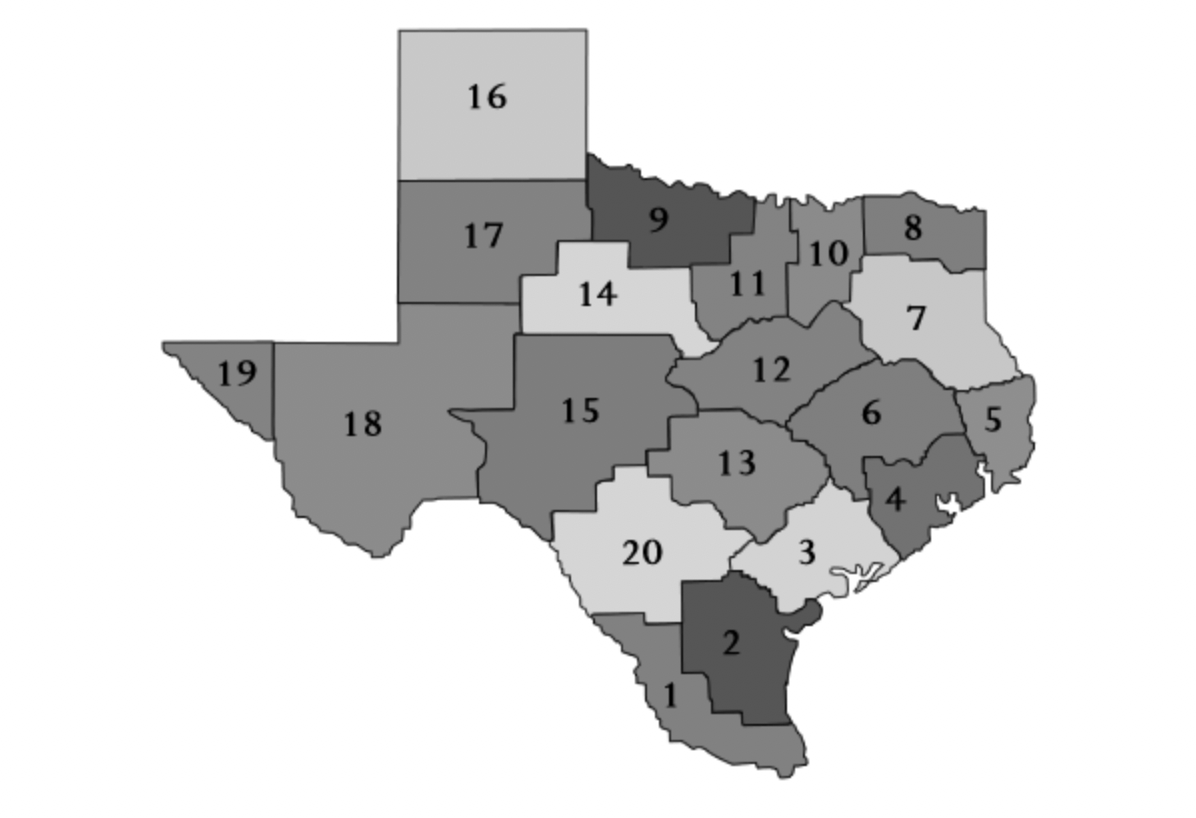
\includegraphics[width=\linewidth]{TEA_regions.png}
\footnotesize
\emph{Note:} Allen ISD is located in region 10. I select control schools from regions 7, 8, 10, 11, and 12.
\end{minipage}
\label{fig:tearegion}
\end{figure}

To determine which districts are similar to Allen, I rely on district types assigned by the National Center for Education Statistics based on the population size of the district and its proximity to urban areas. Since Allen ISD is defined as a "Large Suburb", I filter the sample to only include schools in the same district category. Finally, using 2019 ACS data, I calculate the average commuting time to work in Collin County, TX was 27.7 minutes\footnote{From the 2019 ACS data, I selected households located in Collin County where the head of the household was employed. The commuting time average is weighted using weights assigned by the Census}. I assume anyone within that radius of the location of the raid could have been impacted and remove any school within that boundary. In addition, since Allen ISD is a public school district, I remove all charter schools from the sample. The two strategies help separate difference in performance that were caused by the raid from differences attributable to (1) district-level trends or (2) group-level trends. However, there could still be some concerns that differential trends between schools in Allen ISD and schools that were not exposed to the raid could bias our estimates. For the third difference-in-difference strategy, I address these concerns by using a nearest-neighbor matching procedure to select control schools that are similar to those in Allen ISD. Specifically, from the set of control schools in strategy (2), I calculate propensity scores using three school-level covariates averaged across 2015-2019: the share of Hispanic students, the share of students with limited English proficiency, and the share of economically disadvantaged students. I then measure the difference in propensity scores between the treated and control units and, for each school in Allen, I select the two nearest control schools. Reassuringly, these results are robust to using alternative matching strategies (see \autoref{fig:psmalt}). 


\begin{figure}[!ht]
\caption{{Schools in Allen and site of raid}}
\centerline{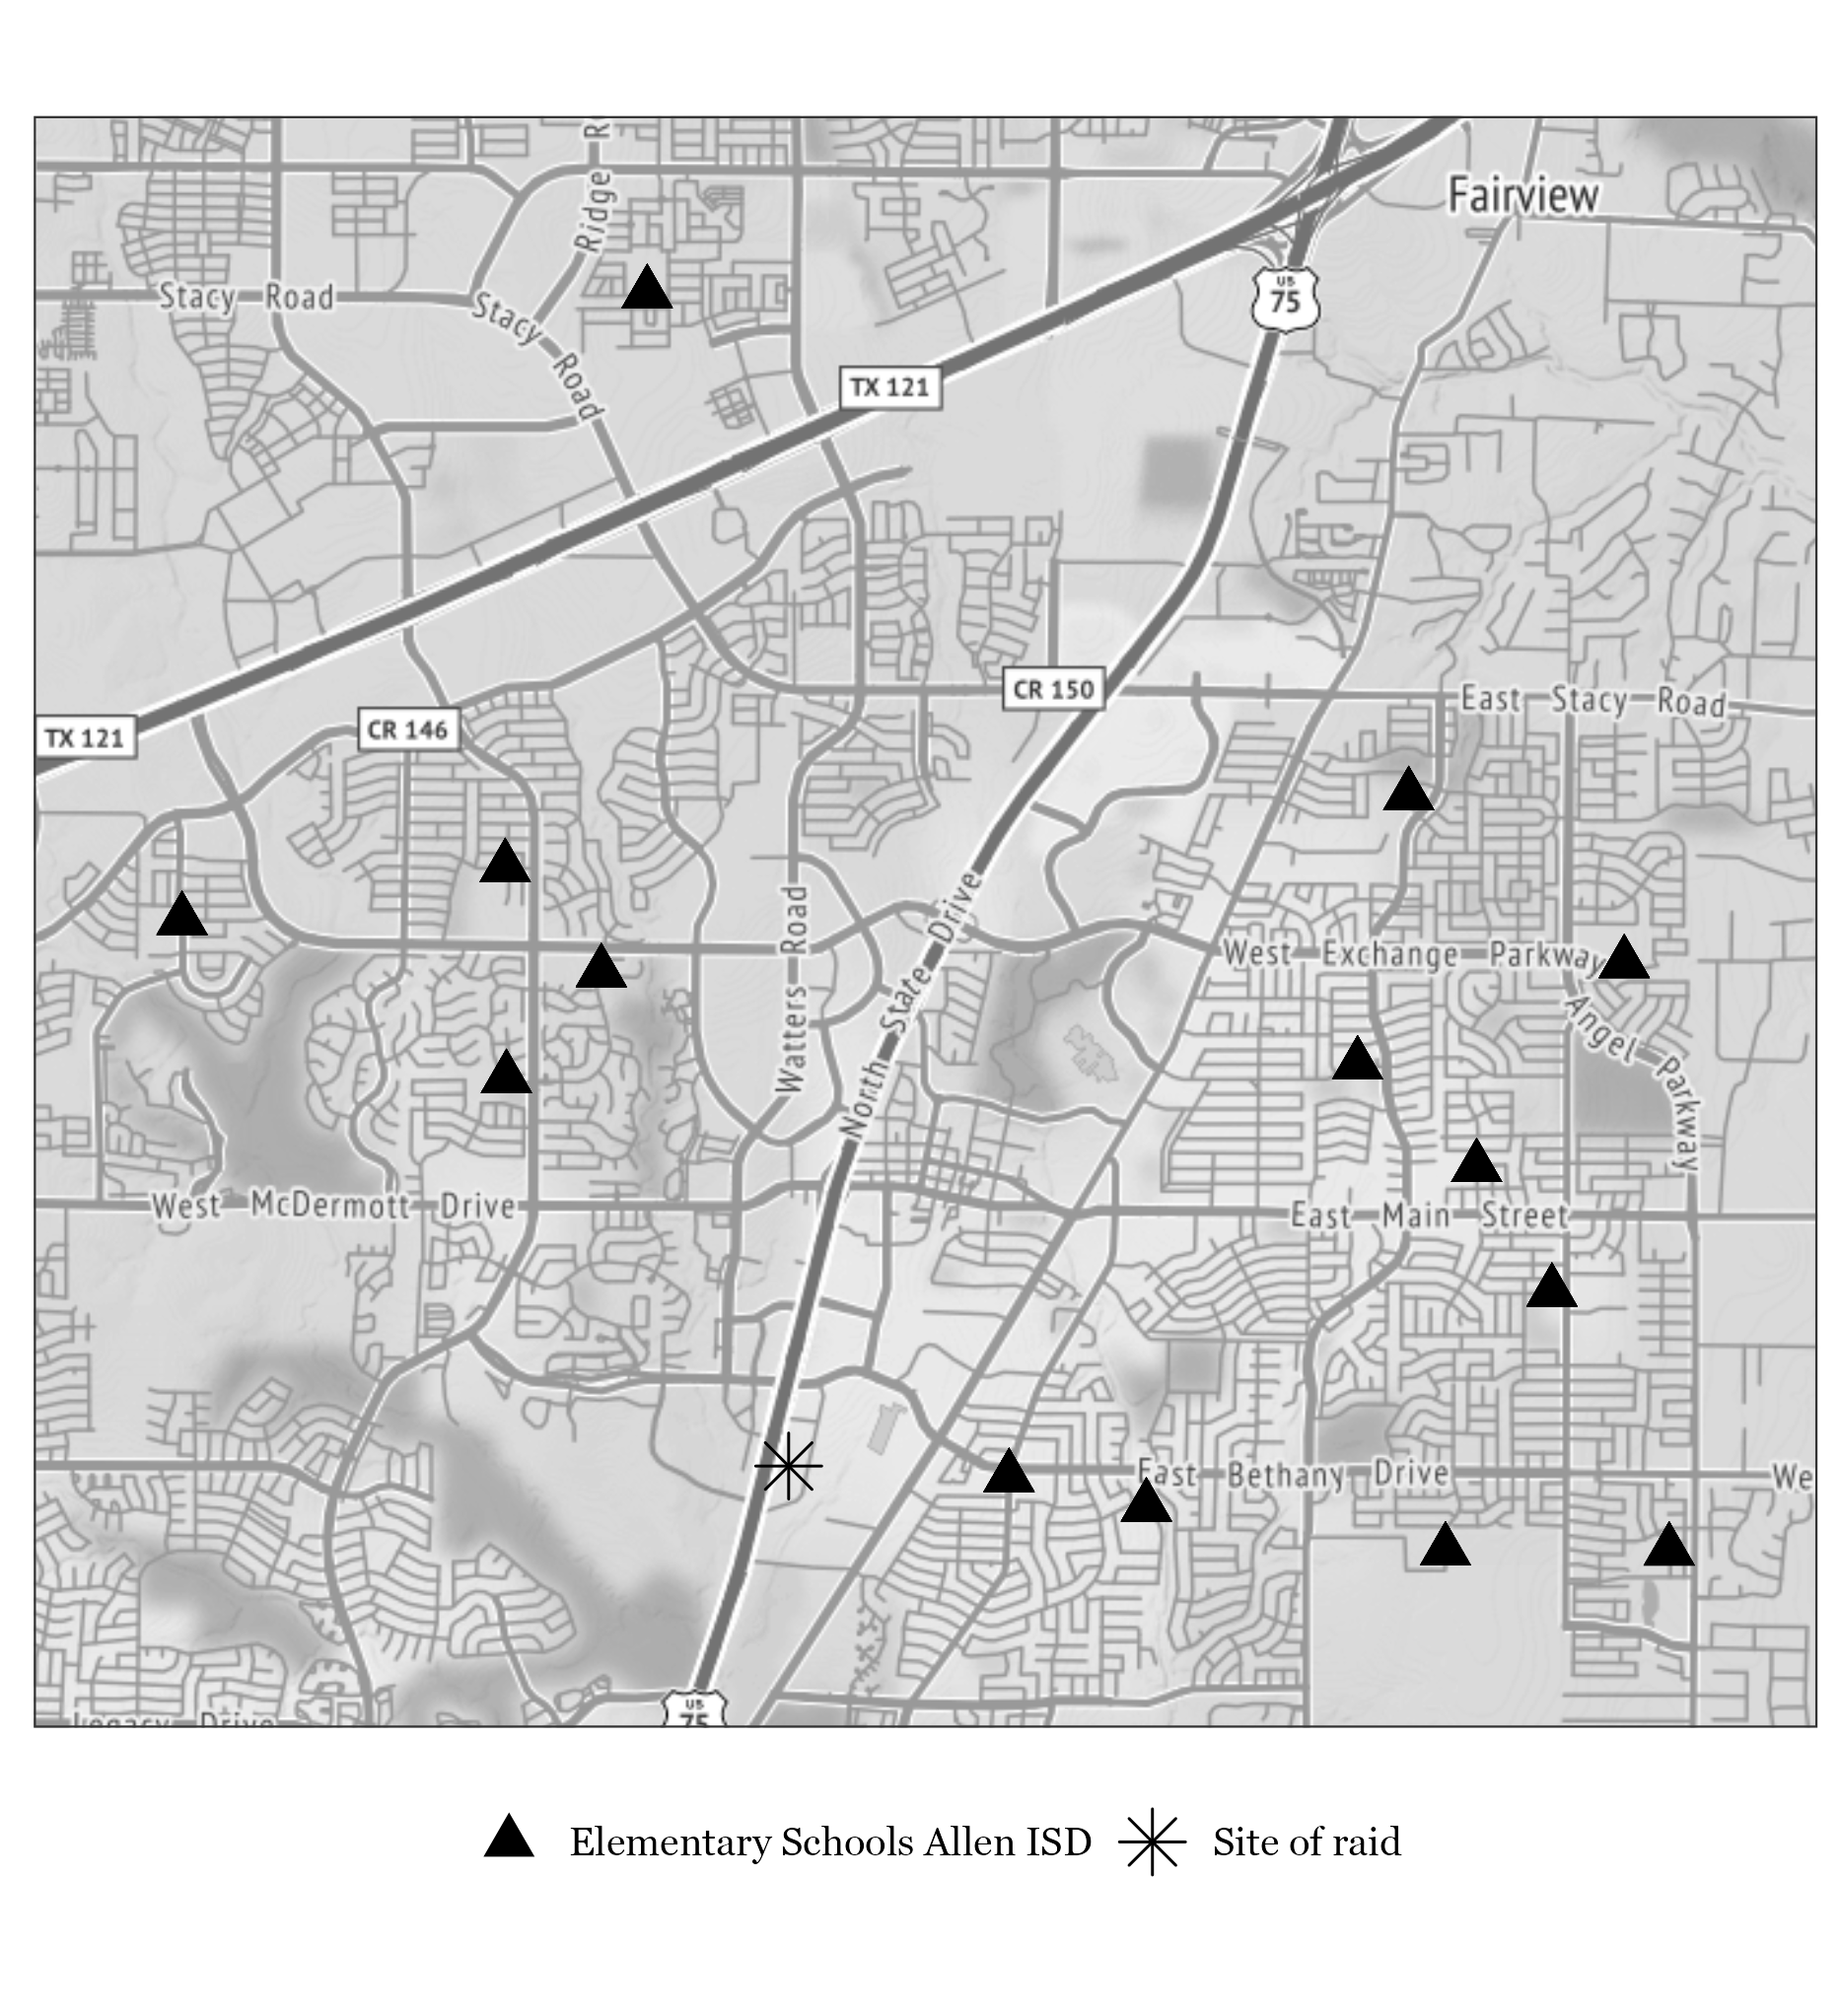
\includegraphics[scale=0.5]{allen_school_map.png}}
\end{figure}

\begin{figure}[!ht]
\caption{{Control schools}}
\centerline{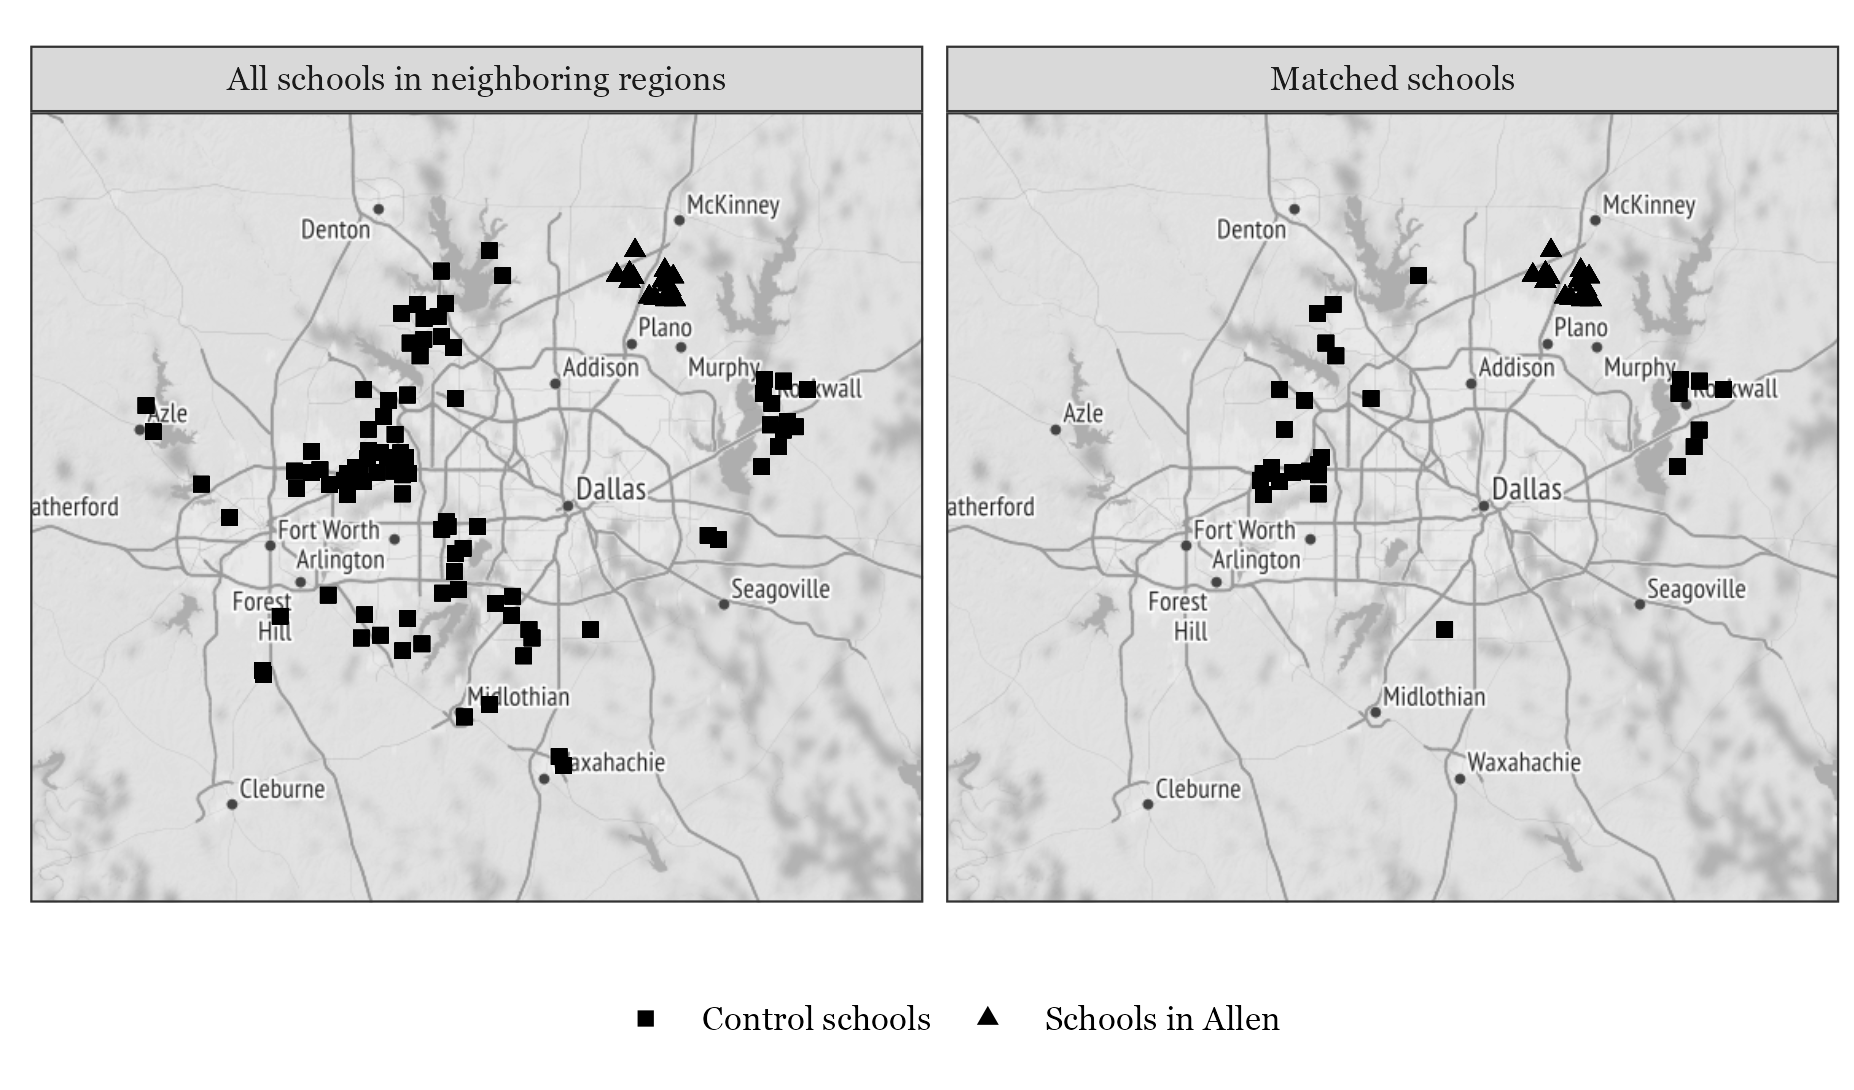
\includegraphics[scale=0.7]{treated_control_school_map.png}}
\end{figure}



\section*{Empirical Approach}

\subsection*{STAAR Test Peformance}

For each control group strategy described above, I  estimate two difference-in-difference regression models. The first model is estimated as follows when using white students in Allen ISD as the control group (1) or Hispanic students in other districts (2):


\begin{equation*}
    y_{rst} = \alpha_{sr} + \omega_{t} + \beta \text{Hispanic}_{r} \times \text{Post}_{t} + \epsilon_{rst}
\end{equation*}
\begin{equation*}
       y_{rst} = \alpha_{sr} + \omega_{t} + \beta \text{Near}_{s} \times \text{Post}_{t} + \epsilon_{rst}
    \end{equation*}

\noindent The dependent variable $y_{rst}$ is defined as the passing rate or the scaled test score in the reading and math test (or a `combined' measure using a weighted average of each subject) for racial-ethnic group $r$ in school $s$ at time $t$. I include a school and racial-ethnic group fixed effect $\alpha$ and time-fixed effect $\omega$. $Hispanic_{r}$ and $Near_{s}$ are indicator variables denoting observations for Hispanic students and for schools that were near the raid (in Allen ISD), respectively. The second model adds time-varying school-level covariates, $\theta_{st}$ including the percent of Hispanic students, the percent of students with limited English proficiency (LEP), and the percent of economically disadvantaged students.

\begin{equation*}
    y_{rst} = \alpha_{sr} + \omega_{t} + \beta \text{Hispanic}_{r} \times \text{Post}_{t} + \theta_{st} + \epsilon_{rst}
\end{equation*}
\begin{equation*}
       y_{rst} = \alpha_{sr} + \omega_{t} + \beta \text{Near}_{s} \times \text{Post}_{t} + \theta_{st} + \epsilon_{rst}
    \end{equation*}

\noindent Finally, for the difference-in-difference-in-differences approach, I use data from white and Hispanic students in Allen as well as in similar districts in neighboring regions. This strategy helps ensure the estimate for the effect of the raid is not biased by other district-wide shocks that affected all students in Allen ISD or by shocks affecting all Hispanic students in Texas. For this, I use the following model:


\begin{equation*}
       y_{rst} = \alpha_{sr} + \omega_{t} + \chi_{1}\text{Hispanic}_{s} \times \text{Post}_{t} + \chi_{2}\text{Near}_{s} \times \text{Post}_{t} + \beta \text{Hispanic}_{s} \times \text{Near}_r \times \text{Post}_{t} +  \theta_{st} + \epsilon_{rst}
    \end{equation*}


\noindent Where $y_{rst}$, $\alpha_{sr}$, $\omega_{t}$, $\theta_{st}$, $Hispanic$, $Post$ and $Near$ are all defined as above. 

\subsection*{Supplemental analyses}

To examine how proximity to the raid was related to the change in students’ academic performance, I use 6th grade scores for Hispanic students from all schools within a 27.7 minute radius of the raid, again relying on ACS data to determine a reasonable cut-off point. Then, I estimate the following simple model:

\begin{equation*}
       y_{s19} - y_{s18} = \beta \text{Distance}_s + \epsilon_{s}
    \end{equation*}

\noindent Where $y_{s19}$ and $y_{s18}$ are the scaled scores and passing rates obtained by Hispanic students in school $s$ in the reading, math, or averaged reading and math tests in 2019 and 2018, respectively. $\text{Distance}_s$ is the estimated time in minutes it would take to drive from school $s$ to the site of the raid. As described above, the Google Maps API does not give users access to historical data on commuting times, so I use the estimated driving time on April 5, 2023 at 8 am (first Wednesday of April like the day of the raid). 

To determine if the raid caused interruptions to schooling, I conduct two analyses. The first uses administrative data on the attendance rates of Hispanic students and follows a similar difference-in-difference approach as the one I used for the STAAR test data. As above, I use Hispanic students in similar school districts and in geographic proximity. Because the attendance rate data pertains to students in all grade-levels in a school, data suppression due to FERPA standards is not an issue, giving me a larger set of eligible control schools. Thus, I am able to restrict the sample to only those schools in the same region as Allen ISD (region 10) rather than relying on neighboring regions. As I do for the STAAR performance analysis, I construct a second control group of Hispanic students in similar schools by matching each treated school to the two nearest control schools based on a nearest-neighbor matching procedure. Then, I estimate two models:

\begin{equation*}
       y_{rst} = \alpha_{s} + \omega_{t} + \beta \text{Near}_{s} \times \text{Post}_{t} + \epsilon_{rst}
    \end{equation*}
\begin{equation*}
    y_{rst} = \alpha_{s} + \omega_{t} + \beta \text{Hispanic}_{r} \times \text{Post}_{t} + \theta_{st} + \epsilon_{rst}
\end{equation*}

\noindent The dependent variable $y_{st}$ is defined as the attendance rate for school $s$ in year $t$. I include a school fixed effect $\alpha_s$ and time-fixed effect $\omega_t$. As in earlier analyses, $Near_{s}$ is an indicator variables denoting schools that were near the raid (in Allen ISD) and $Post_t$ is an indicator denoting observations from the year of the raid (2019). In the second model, I also add time-varying school-level covariates, $\theta_{st}$ including the percent of Hispanic students, the percent of students with limited English proficiency (LEP), and the percent of economically disadvantaged students in school $s$ at time $t$.

Finally, I conduct a second analysis that uses foot-traffic data to measure potential interruptions to schooling. For this analysis, I obtain a similar control group by matching each treated school to another non-charter school in a neighboring region based on the same nearest-neighbor matching procedure. Then, I use a DID event study strategy and estimate the following model:

\begin{equation*}
    \frac{y_{sw}^{19}-y_{sw}^{18}}{y_{sw}^{18}} = \sum_{i=-4}^{-2} \beta_{i} \times Treat_{sw} + \sum_{i=0}^{1} \beta_{i} \times Treat_{sw} + \alpha_{s} + \omega_{w} + \epsilon_{sw}
\end{equation*}

\noindent Where $y_{sw}^{19}$ and $y_{sw}^{18}$ are defined as the number of visits to school $s$ in week $w$ in years 2019 and 2018. $Treat_{sw}$ is an indicator variable set to 1 if school $s$ is in Allen ISD and week $w$ is the same value as $i$. $\alpha_s$ and $\omega_w$ are school and time fixed effects. As described earlier, I use the following weeks for the analysis:

\vspace{2em}
\begin{table}[!htbp] \centering 
  \caption{Weeks Used for Foot Traffic Analysis} 
  \label{} 
\begin{tabular}{@{\extracolsep{5pt}}cll} 
\\[-1.8ex]\hline 
\hline \\[-1.8ex] 
\\Week & 2018 & 2019 \\
\hline \\[-1.8ex] 
-4 & February 26 - March 4 & February 25 - March 3 \\ 
-3 & March 5 - March 11 & March 4 - March 10 \\ 
-2 & March 19 - March 25 & March 18 - March 24 \\ 
-1 & March 26 - April 1 & March 25 - March 31 \\
0 & April 2 - April 8 & April 1 - April 7 \\
1 & April 9 - April 15 & April 8 - April 14 \\
\hline 
\hline \\[-1.8ex] 
\end{tabular} 
\end{table} 

\section*{Results}
\subsection*{STAAR test performance}

\autoref{tab:maineffects} presents the results of the regression model estimating the effect of the raid on the scores and passing rates of Hispanic children in Allen ISD. Across all three control groups, I find significant negative effects on academic performance, with and without school-level time-varying controls. Although there is some variation on the point estimate for magnitude of the effect, on average the scores of Hispanic students decreased by over 30 points. \autoref{fig:performancetrend} presents the raw trends in the scaled scores and passing rates for Hispanic students in Allen ISD and in control groups. The figure provides some evidence to validate the parallel trends assumption in the years prior to the raid and shows sharp decreases in performance following treatment. To further assess this assumption, I also estimate an event study specification (\autoref{fig:performanceeventstudy}) to show these results are robust to the inclusion of group-by-year fixed effects. 

\begin{figure}[!ht]
\caption{{Raw trends in performance across Hispanic students in Allen ISD and control groups}}
\centerline{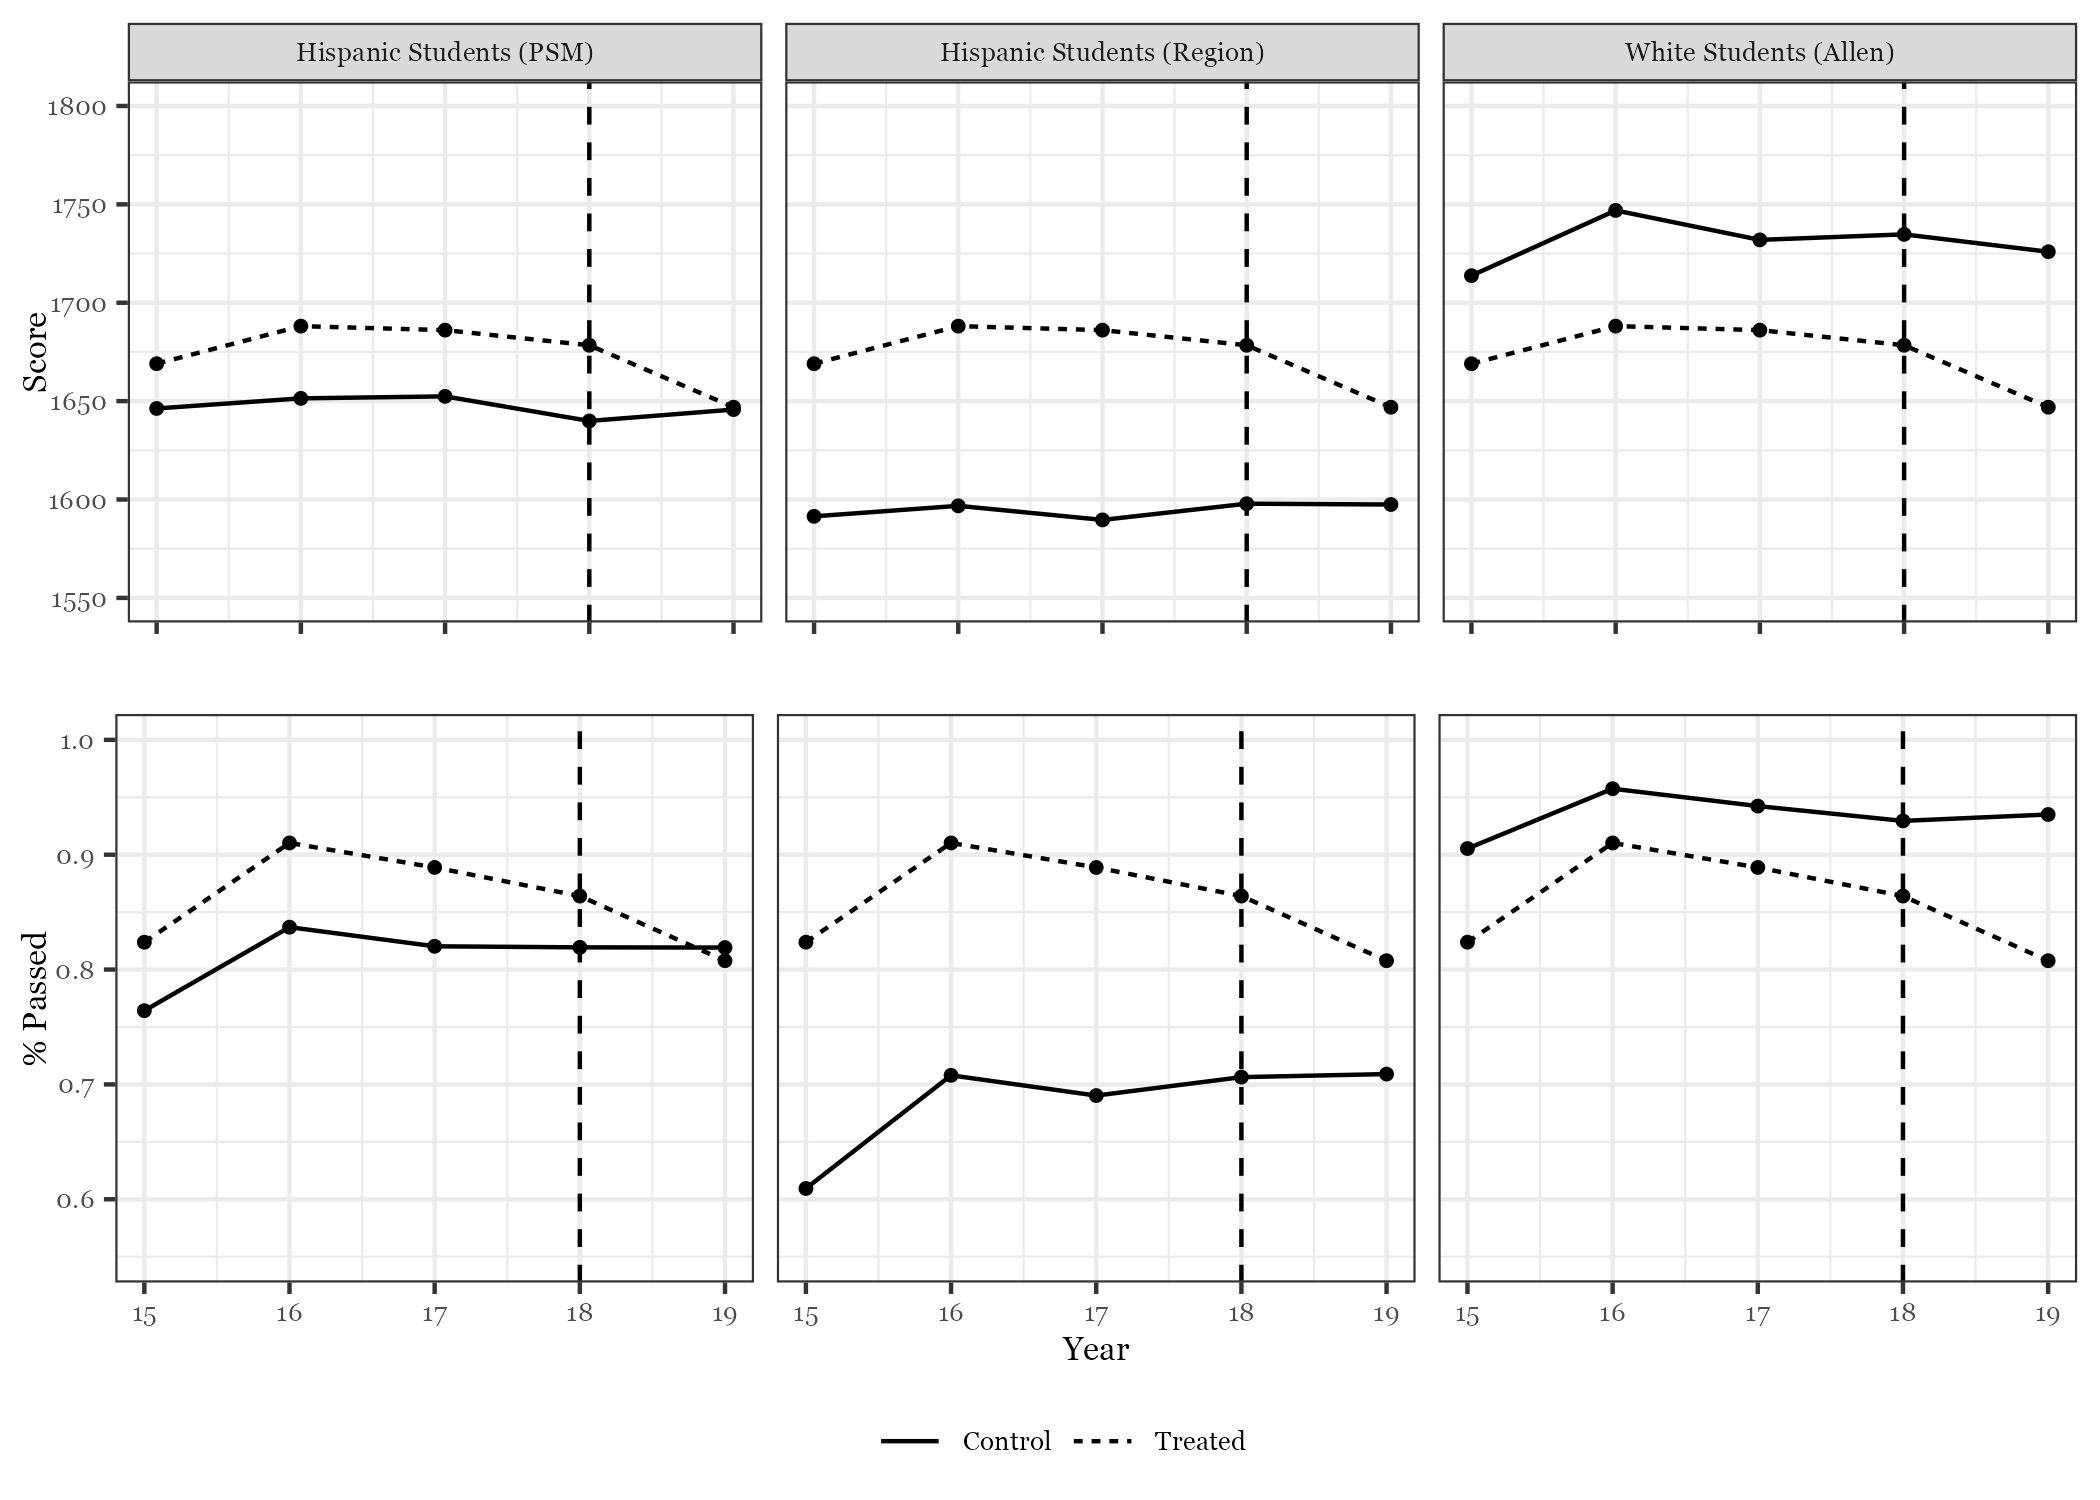
\includegraphics[scale=0.9]{did_trends_combined.png}}
\label{fig:performancetrend}
\end{figure}

\begin{sidewaystable}[!htbp] \centering 
  \caption{Effects of a nearby large-scale workplace raid on academic performance of Hispanic students in Allen ISD} 
  \label{} 
\begin{tabular}{@{\extracolsep{5pt}}lcccccccc} 
\\[-1.8ex]\hline 
\hline \\[-1.8ex] 
\\[-1.8ex] & \multicolumn{6}{c}{DiD} & \multicolumn{2}{c}{Triple Difference} \\ 
 & \multicolumn{2}{c}{White} & \multicolumn{2}{c}{Hispanic (Neighbor Region)} & \multicolumn{2}{c}{Hispanic (PSM)} & \multicolumn{2}{c}{White and Hispanic} \\ 
\hline \\[-1.8ex] 
\\[-2.0ex] \multicolumn{9}{@{} l}{Panel A: Score, math and reading combined}
 \\
 \\[-1.5ex]
 Workplace Raid & $-$32.64$^{**}$ & $-$36.24$^{***}$ & $-$39.73$^{***}$ & $-$43.56$^{***}$ & $-$35.03$^{***}$ & $-$35.79$^{***}$ & $-$32.59$^{**}$ & $-$35.65$^{**}$ \\ 
  & (13.39) & (12.51) & (12.75) & (12.49) & (11.77) & (12.30) & (15.71) & (15.33) \\ 
  & & & & & & & & \\ 
 Constant & 1612.99$^{***}$ & 1686.00$^{***}$ & 1626.81$^{***}$ & 1720.31$^{***}$ & 1626.32$^{***}$ & 1538.23$^{***}$ & 1624.88$^{***}$ & 1696.63$^{***}$ \\ 
  & (10.44) & (115.54) & (10.40) & (31.92) & (9.33) & (83.86) & (11.23) & (20.64) \\ 
  & & & & & & & & \\ 
\\[-1.83ex] 
 \hline \\[-1.83ex]
\\[-2.0ex] \multicolumn{9}{@{} l}{Panel B: Passing rate, math and reading combined}
 \\
 \\[-1.5ex]
 Workplace Raid & $-$7.12$^{***}$ & $-$7.38$^{***}$ & $-$9.86$^{**}$ & $-$10.73$^{***}$ & $-$7.74$^{***}$ & $-$8.15$^{***}$ & $-$9.27$^{**}$ & $-$9.88$^{**}$ \\ 
  & (2.14) & (2.09) & (3.83) & (3.77) & (2.54) & (2.64) & (3.99) & (3.92) \\ 
  & & & & & & & & \\ 
 Constant & 73.32$^{***}$ & 107.23$^{***}$ & 70.01$^{***}$ & 98.92$^{***}$ & 72.01$^{***}$ & 78.99$^{***}$ & 71.64$^{***}$ & 87.91$^{***}$ \\ 
  & (1.67) & (19.31) & (3.12) & (9.64) & (2.01) & (17.97) & (2.85) & (5.28) \\ 
  & & & & & & & & \\ 
\hline \\[-1.8ex] 
School\times  Race FE & \checkmark & \checkmark & \checkmark & \checkmark & \checkmark & \checkmark & \checkmark & \checkmark \\ 
Year FE & \checkmark & \checkmark & \checkmark & \checkmark & \checkmark & \checkmark & \checkmark & \checkmark\\ 
School controls &  & \checkmark &  & \checkmark &  & \checkmark &  & \checkmark \\ 
Observations & 140 & 140 & 540 & 540 & 210 & 210 & 1050 & 1050 \\ 
\hline 
\hline \\[-1.8ex] 
\textit{Note:}  & \multicolumn{8}{r}{$^{*}$p$<$0.1; $^{**}$p$<$0.05; $^{***}$p$<$0.01} \\ 
\end{tabular} 
\label{tab:maineffects}
\end{sidewaystable} 


As the top row of \autoref{fig:performancetrend} shows, the drop in scores widened the gap between Hispanic and white students in Allen ISD and, although these students had consistently performed above their peers in matched schools, the raid fully erased this difference. The historic differences between Hispanic students and white students in Allen ISD are consistent with existing research on achievement gaps across racial-ethnic groups \citep{reardon_2009_the,gandara_2010_the}. These disparities in performance can be particularly consequential in the context of shocks such as a workplace raid because they can push already under-performing students below the passing threshold\footnote{A drop in passing rates is relevant insofar as failing a standardized test can have long-run effects on a student if they are held back a year or on schools if their funding and accountability scores are connected to student performance.}. Indeed, as we see in panel B, the drop in scores was enough to decrease the passing rate of Hispanic students in Allen by around 8 percentage points. If Hispanic students in Allen had been performing at the level of their white counterparts, the drop in scores would have led to fewer students failing the test. Conversely, if the raid had affected lower performing schools in the region, these schools would have likely seen larger impacts on their students' passing rates, even if the baseline effects on scaled scores were the same. This emphasizes the point that existing educational disparities make already vulnerable groups less resilient to shocks that might impact academic performance. As an illustration, in \autoref{fig:simchanges} I show how the change in passing rates from 2018 to 2019 might have been different if Hispanic students in Allen ISD had been performing at the higher level of white students in the district or the lower level of other Hispanic students in neighboring regions\footnote{To construct \autoref{fig:simchanges}, I use historical STAAR score conversion tables to find the score corresponding to the passing threshold for the given testing year. Using the school-level data on the percent of Hispanic students who passed the test and their average score, I make the assumption that student scores are normally distributed around this average and find the standard deviation that models the observed distribution. Then, to simulate the change in passing rates if Hispanic students in Allen had been performing at the level of white students or Hispanic students in neighboring districts, I keep the same standard deviation but increase or decrease the mean based on the average difference between the two groups in pre-treatment years.}. 


\begin{figure}[!ht]
\caption[]{Simulated changes in passing rates for different levels of academic performance}
\centerline{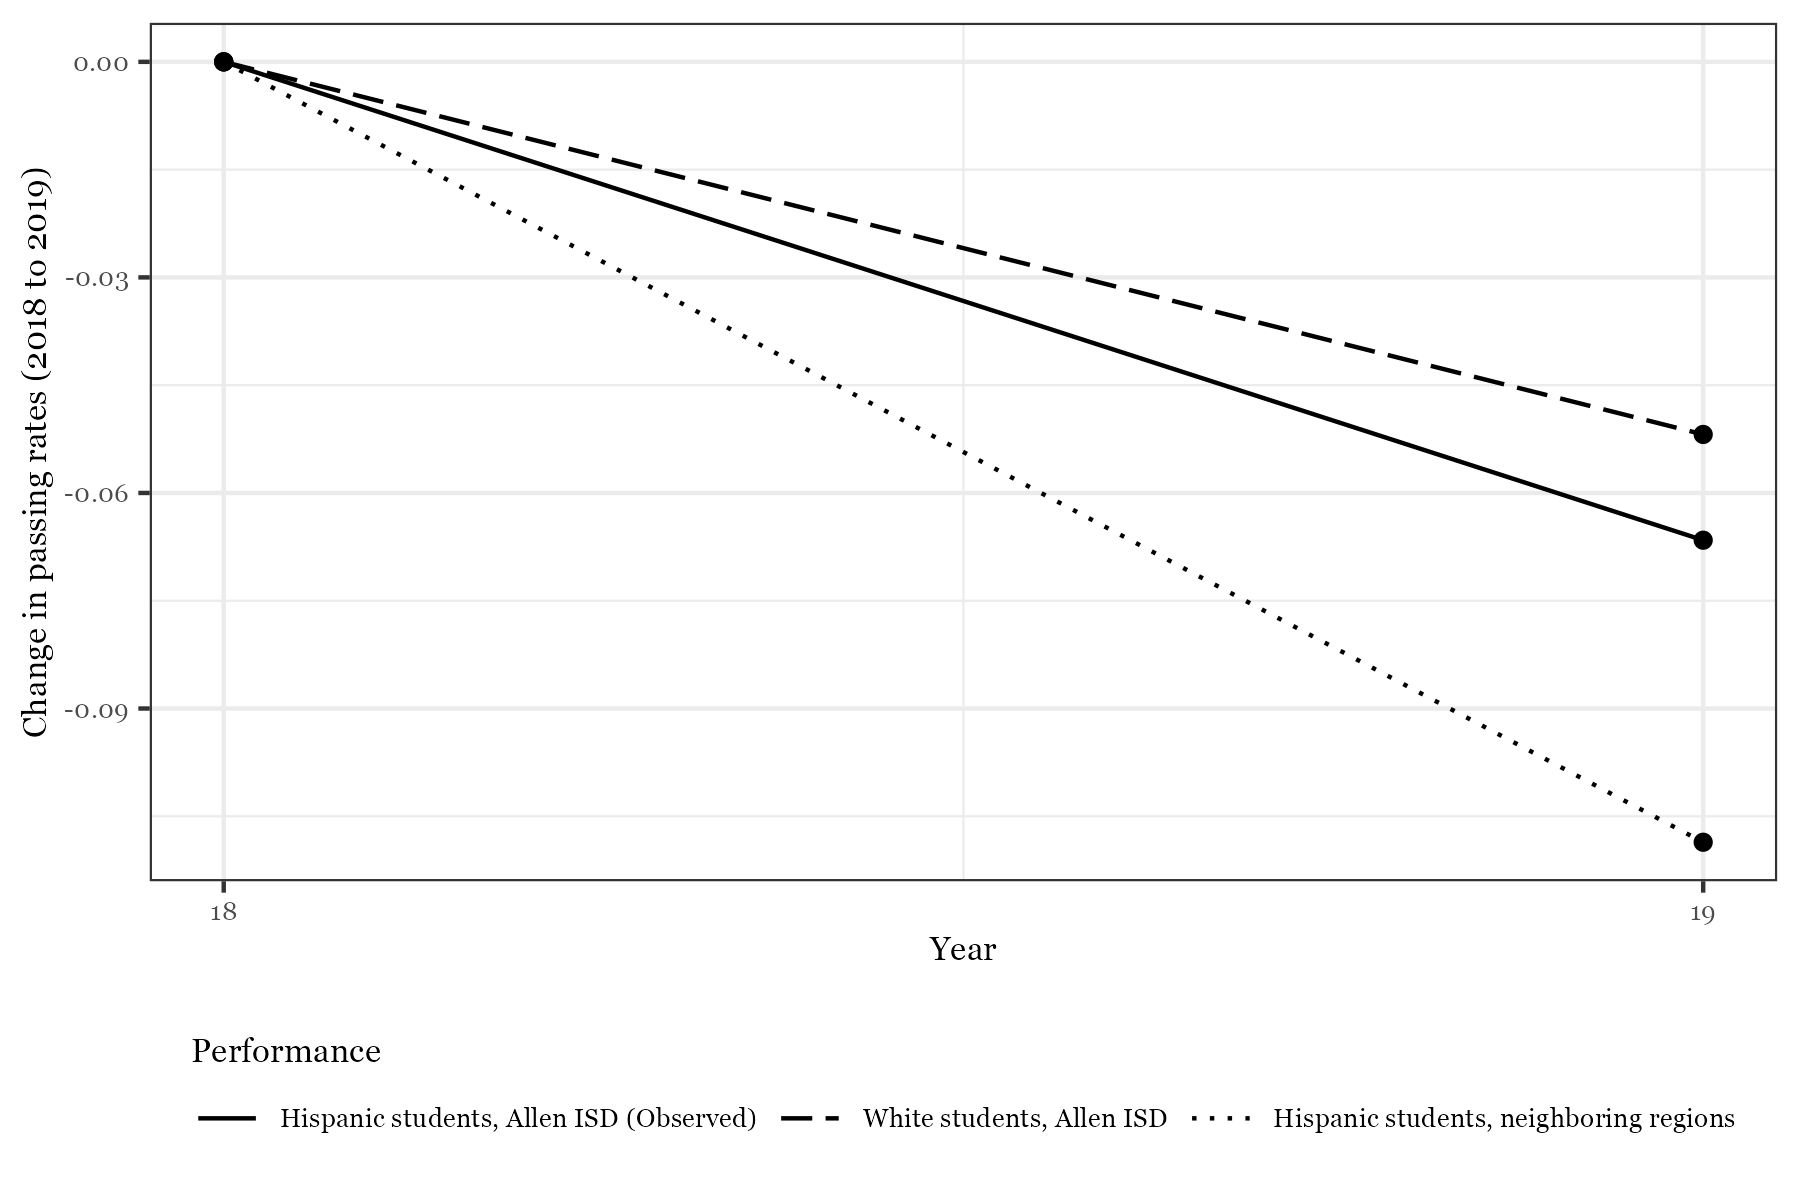
\includegraphics[scale=0.7]{differences_passing_rate_drop.png}}
\label{fig:simchanges}
\end{figure} 


\subsection*{Supplementary Analyses}

In all the analyses above, I assume Hispanic students in all schools in Allen ISD were exposed to the raid and experienced the same level of treatment. However, the distance of the school from the raid is an important potential source of heterogeneity in the effects of the raid. \autoref{tab:distance_eff} shows the results of the model regressing the change in scores and passing rates from 2018 to 2019 on the estimated commuting time from the school to the raid, in minutes. I find that distance has a significant positive effect on the change in passing rates and scores, indicating that proximity to the raid was predictive of a larger drop in performance. For each minute further away from the raid, the change in score and passing rates increases by an average of 1.74 points and 0.35 percentage points, respectively. On average, a school one minute from the raid would be expected to see a 5.8 percentage point drop in their passing rate and 35.35 drop in scores. By contrast, a school 15 minutes away from the raid would be expected to have a minimal change in their passing rates (-0.55 percentage points) and about a 9.2 drop in scores. \autoref{fig:distanceperformance} in the appendix presents these results graphically. 


\begin{table}[!htbp] \centering 
  \caption{Relationship between the distance of a school to the raid and the change in student performance from 2018 to 2019} 
  \label{} 
\begin{tabular}{@{\extracolsep{5pt}}lcc} 
\\[-1.8ex]\hline 
\hline \\[-1.8ex] 
\\[-1.8ex] & \multicolumn{2}{c}{} \\ 
 & Score & Passing Rate \\ 
\hline \\[-1.8ex] 
 Minutes from raid & 1.740$^{***}$ & 0.354$^{***}$ \\ 
  & (0.550) & (0.134) \\ 
  & & \\ 
 Constant & $-$35.347$^{***}$ & $-$5.859$^{**}$ \\ 
  & (10.522) & (2.559) \\ 
  & & \\ 
\hline \\[-1.8ex] 
Observations & 156 & 156 \\ 
\hline 
\hline \\[-1.8ex] 
\textit{Note:}  & \multicolumn{2}{r}{$^{*}$p$<$0.1; $^{**}$p$<$0.05; $^{***}$p$<$0.01} \\ 
\end{tabular} 
\label{tab:distance_eff}
\end{table} 

\noindent There are a few potential reasons why the distance between a school and the raid could mediate the effects of the raid on academic performance. First, if workers impacted by the raid lived in the nearby community, then students in the nearest schools were more likely to know someone impacted by the raid. Such a direct exposure to the raid would increase stress due to concern for family and community members and could produce a heightened sense of threat for their own well-being. Moreover, if a parent or close member of their community was detained, it could lead to strong disruptions in their home life and impact their academic performance directly by causing them to miss school and affecting their homework and after-school routines. But even if the 6th graders in nearby schools did not know anyone detained, the proximity to the raid could still affect the extent and type of exposure these students had to the event. Those closest to the raid were more likely to physically witness the operation, seeing or hearing the hundreds of ICE agents that came to the location, some by helicopter. Second, because geography and neighborhoods shape networks of communication, those living close to the raid might have been more likely to hear first-hand experiences of the raid, as compared to students in more distant schools who might have only learned about it through news media. 

If the drop in performance can be attributed to disruptions to schooling, we might expect to see some effect on the attendance rate of Hispanic students. \autoref{tab:attendancerate} shows the results of the difference-in-difference analyses estimating the effects of the raid on Hispanic students' attendance rate in Allen ISD. Estimates for the drop in attendance rate range from a 0.188 percentage point drop to a 0.268 drop. 


\begin{table}[!htbp] \centering 
  \caption{Effects of a nearby large-scale workplace raid on the attendance rate of Hispanic students in Allen ISD} 
  \label{} 
\begin{tabular}{@{\extracolsep{5pt}}lcccc} 
\\[-1.8ex]\hline 
\hline \\[-1.8ex] 
\\[-1.8ex] & \multicolumn{4}{c}{} \\ 
 & \multicolumn{2}{c}{Hispanic (Neighboring Region)} & \multicolumn{2}{c}{Hispanic (PSM)} \\ 
\hline \\[-1.8ex] 
 Workplace Raid & $-$0.188$^{*}$ & $-$0.220$^{**}$ & $-$0.253$^{**}$ & $-$0.268$^{**}$ \\ 
  & (0.102) & (0.107) & (0.125) & (0.131) \\ 
  & & & & \\ 
 Constant & 97.287$^{***}$ & 98.486$^{***}$ & 97.265$^{***}$ & 99.364$^{***}$ \\ 
  & (0.153) & (0.516) & (0.168) & (0.765) \\ 
  & & & & \\ 
\hline \\[-1.8ex] 
School FE & \checkmark & \checkmark & \checkmark & \checkmark \\
Year FE & \checkmark & \checkmark & \checkmark & \checkmark \\
School controls &  & \checkmark &  & \checkmark \\
Observations & 655 & 655 & 300 & 300 \\ 
\hline 
\hline \\[-1.8ex] 
\textit{Note:}  & \multicolumn{4}{r}{$^{*}$p$<$0.1; $^{**}$p$<$0.05; $^{***}$p$<$0.01} \\ 
\end{tabular} 
\label{tab:attendancerate}
\end{table} 


\begin{figure}[htbp]
\caption{{Trends in attendance rate of Hispanic students 2015-2019}}
\centerline{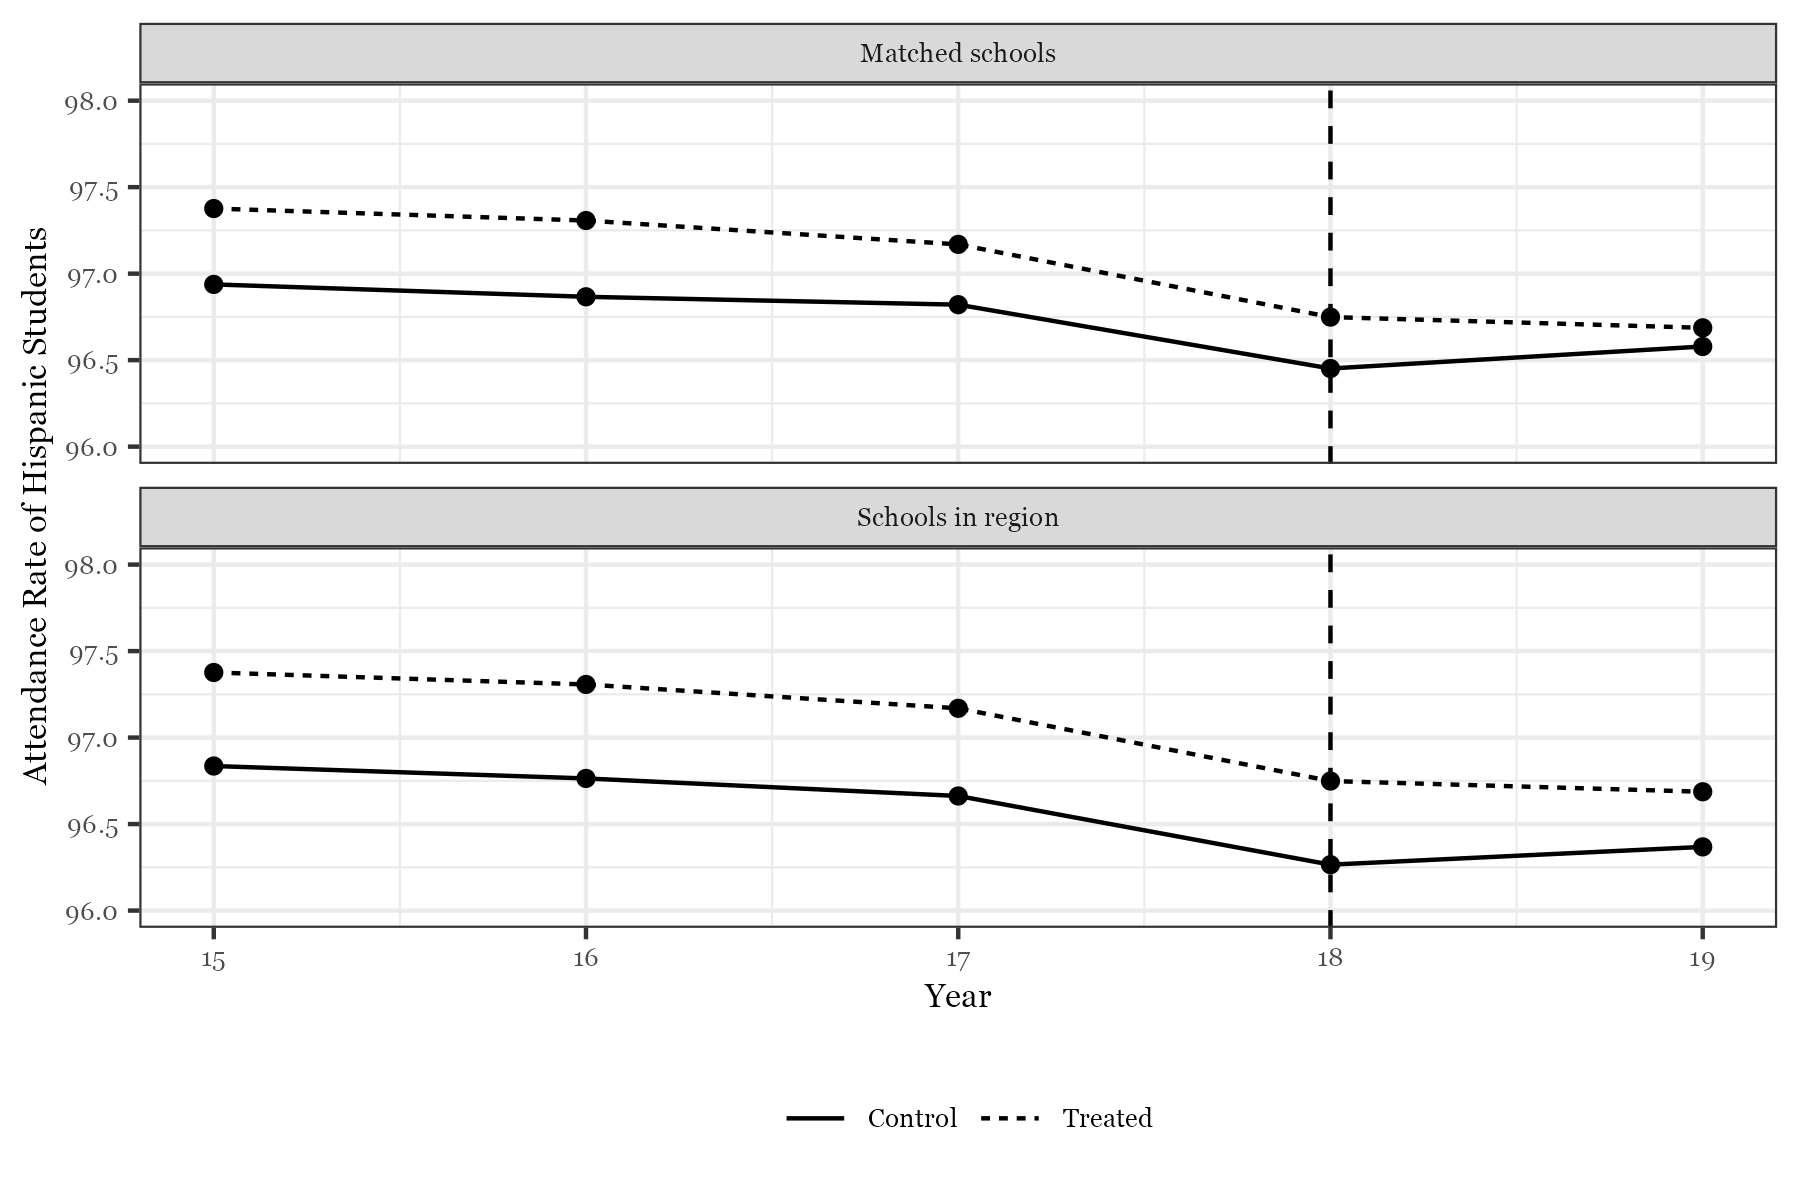
\includegraphics[scale=.7]{did_trends_attendance_rate.png}}
\end{figure}

As described earlier, the TEA measures attendance rate as the total number of days students were present over the total number of days students were in membership at the school. In 2019, Allen ISD had 175 days of instruction. If we assume most students maintained membership for the duration of the academic year, the effects on attendance rate would translate to an average of 0.329 to 0.469 additional missed days of school for Hispanic students. Although it is likely the effects on attendance rate were concentrated on a subset of Hispanic students who faced deeper disruptions, the decrease in attendance is probably too small to conclusively identify it as a mechanism driving down academic performance. 

When I estimate disruptions to schooling using foot traffic data, I am unable to detect any effects. In \autoref{tab:foottraffic} below, the percent change in foot traffic in the week prior to the raid (Week = -1) is used as the reference period. In the week of the raid and the following week, there is no significant change in the number of visits to school in Allen ISD as compared to the same week in 2018. \autoref{fig:foottraffic} shows the number of visits relative to 2018 follows the same patterns for schools in Allen ISD as well as for untreated schools in the neighboring regions. 

\begin{table}[h]
\caption{\% change in foot traffic 2018-2019 in weeks before and after the raid}
\vspace{-2em}
\centering
\begin{tabular}{lc}
   \tabularnewline \midrule \midrule
   & Matched schools in neighboring regions \\
   \midrule
   Allen ISD $\times$ Week $=$ -4    & 0.0213\\   
                                            & (0.1076)\\   
   Allen ISD $\times$ Week $=$ -3    & -0.1032\\   
                                            & (0.0964)\\   
   Allen ISD $\times$ Week $=$ -2    & 0.0043\\   
                                            & (0.1041)\\   
   Allen ISD $\times$ Week $=$ 0     & -0.0504\\   
                                            & (0.0700)\\   
   Allen ISD $\times$ Week $=$ 1     & -0.0514\\   
                                            & (0.0844)\\   
   \midrule
   School FE                                   & \checkmark\\  
   Week FE                                     & \checkmark\\  
   Observations                             & 252\\  
   \midrule \midrule
\end{tabular}
\label{tab:foottraffic}
\end{table}

\begin{figure}[htbp]
\caption{{Trends in foot traffic}}
\vspace{-2em}
\centerline{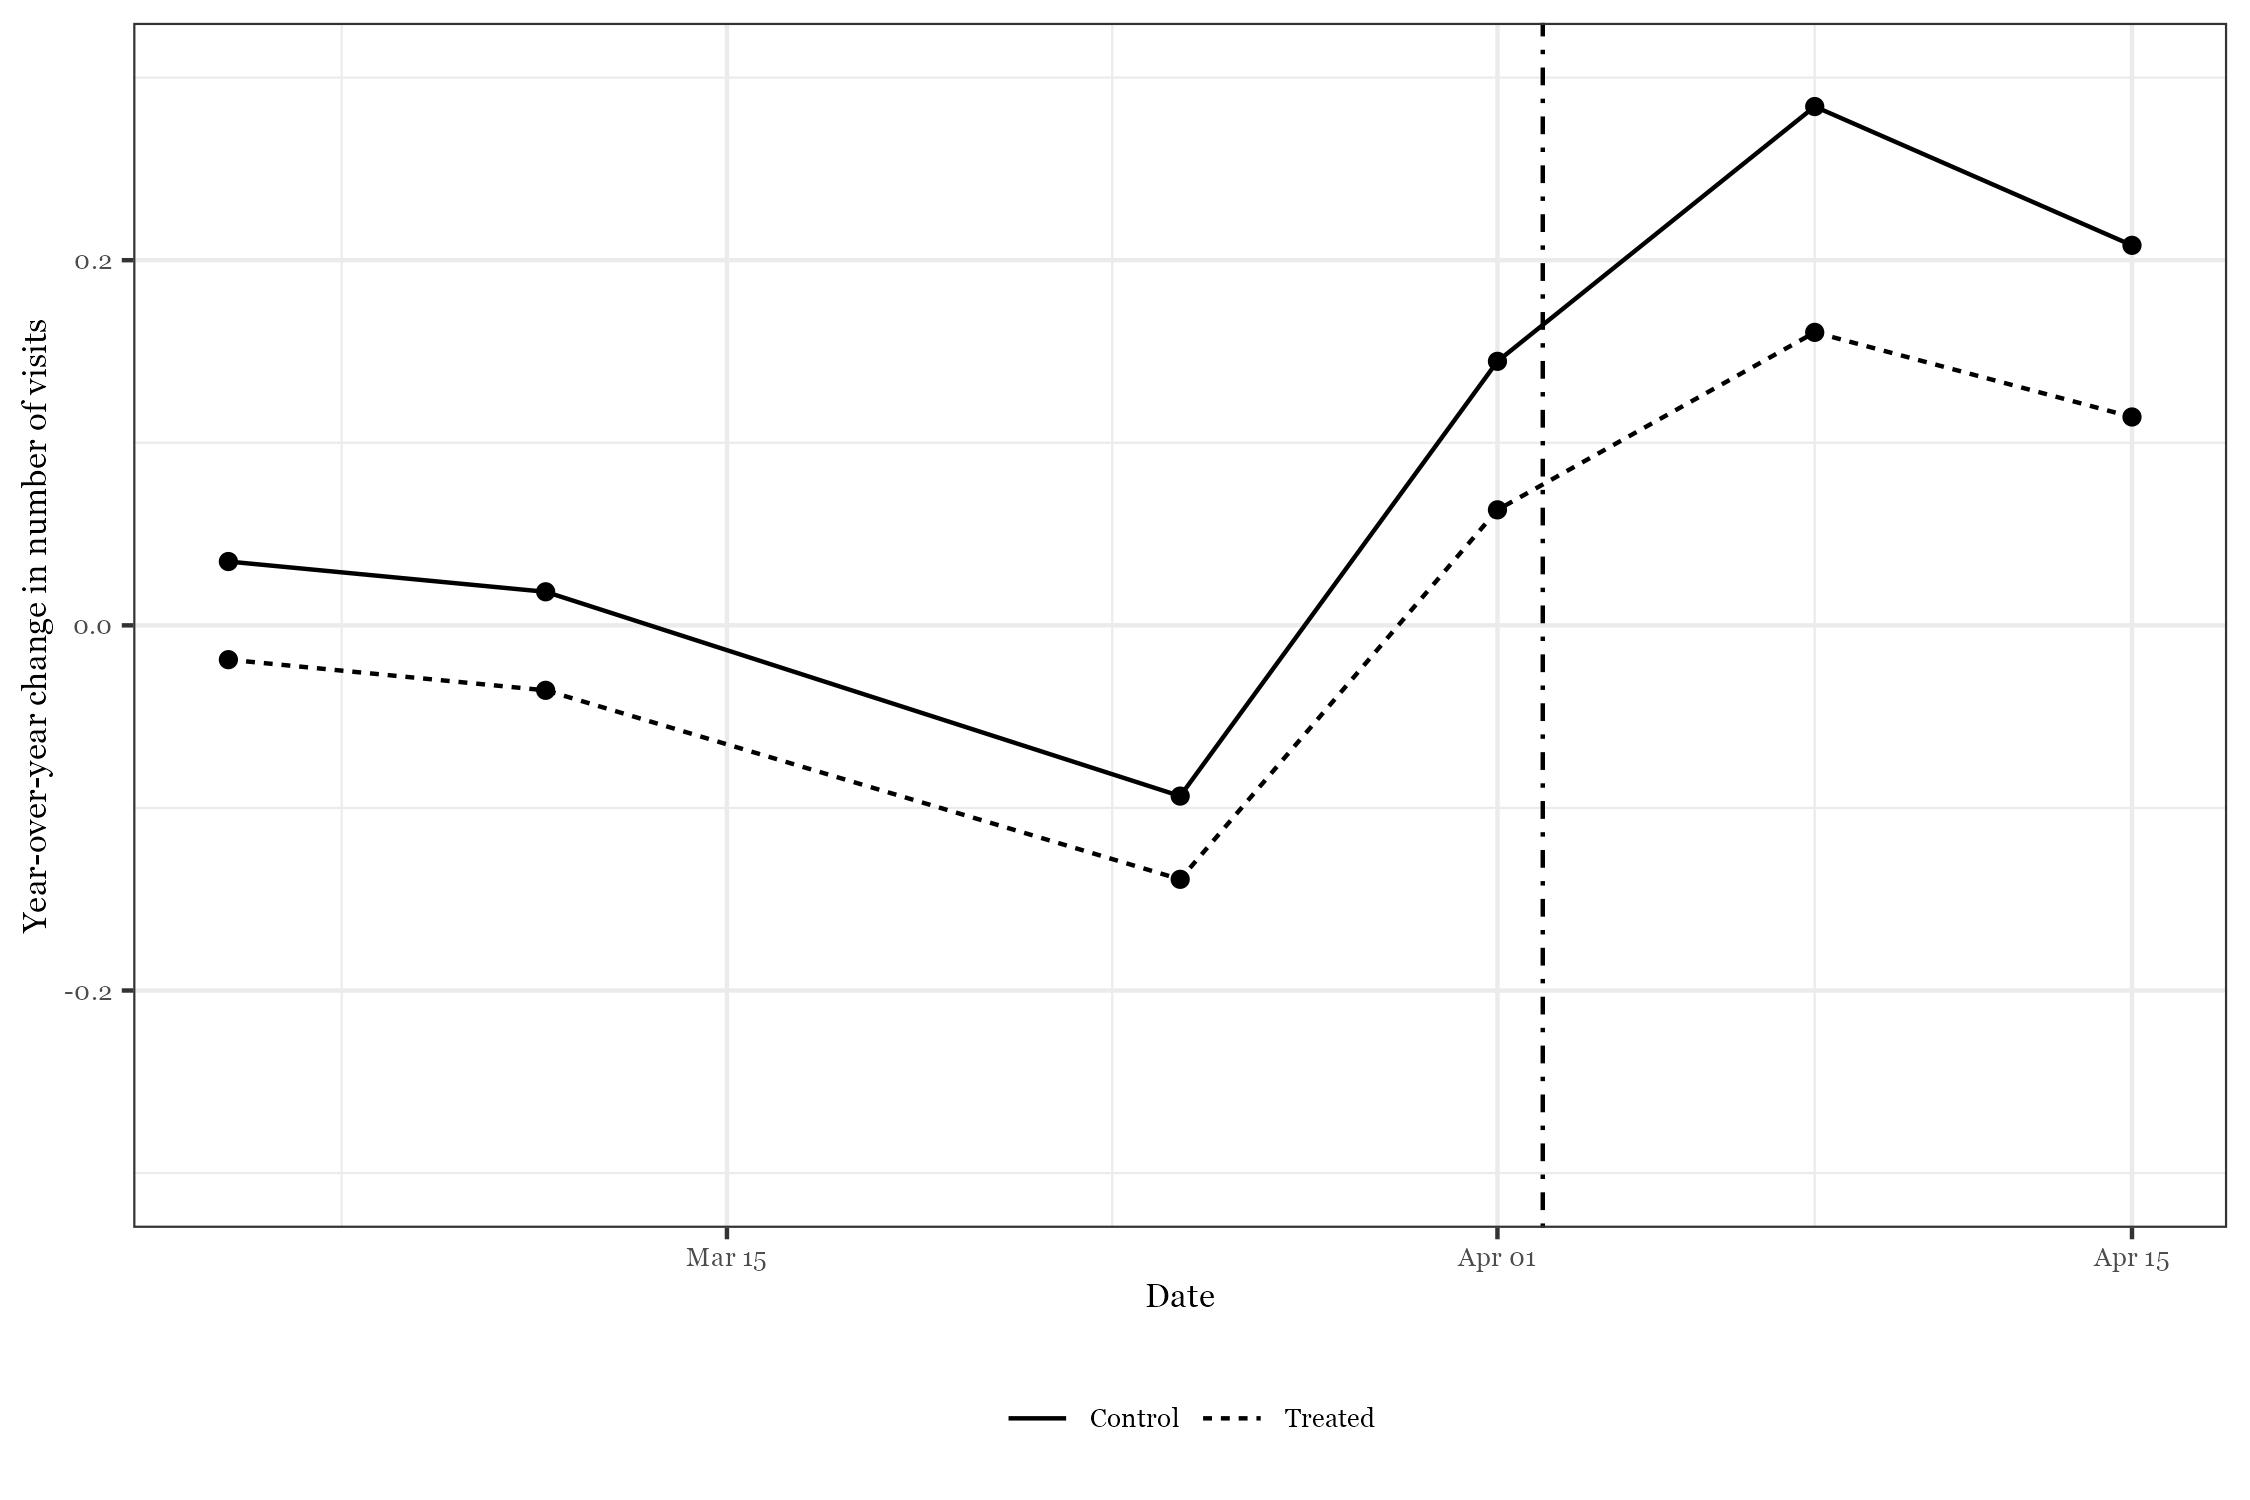
\includegraphics[scale=.6]{safegraph_visit_trends.png}}
\label{fig:foottraffic}
\end{figure}

Overall, while there might have been disruptions to schooling, the analyses suggests these effects might have been too small to lead to the large drops I find in academic performance.


\section*{Discussion}

The use of work-site raids to enforce immigration law has see-sawed over the last 20 years, rising sharply during republican presidential administrations and falling when democrats are in office. Indeed, in October 2021, the Biden administration announced it would halt large-scale workplace immigration raids and focus its enforcement efforts on employers rather than individual workers \citep{Sullivan2021Oct}\footnote{This policy was part of a larger plan to reverse Trump-era immigration restrictions, including lifting visa restrictions, protecting the Deferred Action for Childhood Arrivals program, and ending the ``Remain in Mexico" policy \citep{apnews,krogstad_gonzalez-barrera_2022}. However, by 2023 few of these plans had been realized and the administration even extended restrictive immigration policies set during the Trump presidency despite promises to the contrary \citep{Rose2022Jan}.}. However, because the decision to use work-site raids remains largely at the discretion of the DHS director, we could see this practice re-instituted in the coming years. 

Workplace raids have long been criticized for causing physical and psychological harm to workers and their children while doing little to reduce undocumented migration \citep{tennessee_2019_tirrc,capps_2007_paying,capps_2015_implications,kitroeff_2018_workplace,juby_2011_postville}. Despite controversies around this practice, there has been little causal research on the spillover effects of worksite raids on children's education. On-the-ground reports provide anecdotal evidence that raids lead to interruptions to schooling and decrease academic performance as children grapple with the emotional distress of the raids \citep{capps_2007_paying,chaudry_2010_children} but do not give us actual estimates for the causal effects of the raid. Similarly, we know 287(g) agreements decrease average achievement for Hispanic students in English Language Arts \citep{bellows_2019_immigration}, decrease attendance \citep{bellows_2021_the}, and displace Hispanic students \citep{dee_2019_vanished}, but unlike worksite raids, 287(g) programs deliver more prolonged and often less visible shocks to immigrant communities, likely impacting academic performance in distinct ways. As such, understanding the impact of worksite raids on academic performance bridges an important gap in the literature. 

In this paper, I used data from standardized tests in Texas to present the first causal evidence that exposure to a workplace immigration raid lowers academic performance. Using a variety of difference-in-difference and triple difference strategies, I find a workplace raid conducted in Allen, Texas led to a 7-10 percentage point decrease in the combined math and reading passing rates and a 33-44 point decrease in score. In addition, I find schools close to the raid experienced larger drops in performance but do not find strong evidence to suggest drops in performance were caused by interruptions to schooling. 

These results complement existing research on the spillover effects of immigration enforcement, providing additional evidence that the impact of enforcement and removal operations is not confined to those deported but can also affect Hispanic children in the community. In addition, this research illustrates how a shock in the neighborhood or family environment can reverberate through other social institutions, affecting the child's academic performance and potentially creating long-lasting disruptions to their educational trajectory. The findings thus lay bare the precarious journey children of immigrants must navigate as they transition to adulthood. Not only are they more likely to experience shocks in their neighborhood and family environment but, because the school they attend are also likely to have limited resources, the institution might do little to prevent these shocks from impacting their education. Moreover, existing racial and ethnic achievement gaps mean Hispanic students are already scoring at a lower level than their white peers and any decreases in academic performance is more likely to put them below a passing threshold, creating further consequences. 

This work can give educators insights into the potential short-term effects of the raid and inform practices set in place by school districts to allow for a better coordination among the school, family, and neighborhood institutions. In the wake of a large-scale immigration enforcement, schools could direct additional resources towards Hispanic students in order to compensate for the shock caused by the operation, potentially helping lessen a longer-term achievement gap. In addition, state and district administrators can grant leniency when assessing the academic performance of affected schools to determine their ratings, just as the Texas Education Agency did throughout the COVID-19 pandemic \citep{tea_2020_sb1365}.

Despite these contributions, there are several limitations to the study. First, although I find stronger effects in schools closer to the raid, I am unable to determine why these students are most affected. One possibility could be related to the type of exposure. Those closest to the raid were likely to physically witness the operation which could have triggered a different stress response than hearing about a raid on the news or through word-of-mouth. An alternative explanation relates to neighborhood and community boundaries. First, students living in communities close to the raid are probably more likely to know someone impacted by the operation. This can affect their academic performance directly–perhaps because they had to miss school or had other disruptions in their class and homework schedule–or indirectly by causing emotional distress. Second, the distance from the raid can impact communication networks, making those outside of a narrow radius less likely to hear about the raid. Here, it would be important to also gather data on news coverage in TV and radio stations outside of Allen to estimate the level of media exposure faced by students and parents further from the raid. Finally, community boundaries could influence the effects of legal violence by determining whether an individual identifies with the victim. Studying the effect of neighborhood shootings on cognitive performance, Sharkey \citep{sharkey_2010_the} finds decreases in the scores of of Black but not Hispanic students. He hypothesizes the homicides may have been less salient or threatening for Hispanics because the victims were majority Black. While my analysis only considers the scores of Hispanic students, different Hispanic communities can have significant demographic, socioeconomic, or immigration status differences. These factors can create distinct identities that influence how students in different geographies identify themselves or their families with the violence.

In particular, the immigration status of the student and parents might play an important role in determining whether legal violence feels threatening or salient. While violence perceived as deviant from mainstream social activity, such as a shooting in one's neighborhood, can create a general feeling of danger, state-sponsored legal violence might only threaten those in a precarious immigration status. Previous research on legal violence and health has found divergent answers to this question: Novak \citeyearpar{novak_2017_change} shows an immigration raid in Iowa increased the risk of low-birthweight even among US-born Latina mothers, but Torche \& Sirois \citeyearpar{torche_2019_restrictive} find the enactment of a restrictive immigration bill only impacted Latina immigrant mothers and not their US-born counterparts. Although public TEA data did not allow me to consider the nationality or immigration status of Hispanic students and their parents, country of birth and immigrant status can play mediating roles in how an individual is affected by exposure to legal violence. Future research on immigration enforcement and education should take this into consideration.

In addition to exploiting variations in the geographic proximity of schools to the raid, future research could also use variation in the time between other raids and a state's standardized testing dates to understand how long the academic effects of legal violence persist. Because of disruptions related to the COVID-19 pandemic, I could not explore how the impact of LSWRs on Hispanic students' performance changed in later testing years, so these findings are limited to the 40 days following a raid. Previous research on violence finds the adverse effects of local homicides on older adolescents' attention fade after a week to 10 days \citep{sharkey_2010_the}, so it would be useful to apply this research design to other worksite raids and exploit variations in their timing relative to testing to better understand how enduring these effects might be. Complementing this research with interviews with educators and community members could help us better understand why effects might have persisted beyond those predicted by prior research.

These limitations notwithstanding, these findings provide policymakers with concrete evidence that workplace raids don't just target undocumented workers but have harmful effects on children in the community, including those with legal standing in the country. While deportations of any kind are likely to impact the families and communities of undocumented immigrants, the militaristic and large-scale nature of work-site raids might be particularly traumatic and cause the large spillover effects I detect in these analyses. Understanding the social implications of this kind of immigration enforcement can help inform the priorities and guidelines set out by DHS and provide strong motivation for discontinuing these harmful practices altogether. 


\clearpage

\bibliography{effects_workplace_raids}
\bibliographystyle{apacite}

\clearpage


\section*{Appendix}
\subsection*{Supplementary Methods}
\subsubsection*{Individual math and reading scores}

In all the analyses above, I use a measure for the passing rate and scaled score of students that combines their performance in the math and reading test. Specifically, for each school $s$ and year $t$, I calculated the following measure:

\begin{equation*}
    Y_{\text{Combined}} = \frac{Y_{\text{Reading}} \times N_{\text{Reading}} + Y_{\text{Math}} \times N_{\text{Math}}}{N_{\text{Reading}} + N_{\text{Math}}}
\end{equation*}

\noindent Where $Y$ is either the scaled score or the passing rate in the STAAR test and $N$ refers to the number of students taking each test. Although the main results use the combined measure, I also performed each of the analyses on the individual math and reading tests. \autoref{tab:maineffects_subject} shows the results of the main difference-in-difference and triple difference models using the same control groups described above. The direction and magnitude of the effect is similar for both subjects, although the estimate of the effect on the math test is larger in most of the models. These results run contrary to previous research on the effects of community violence and aggressive policing on academic performance which show larger effects on reading assessments and smaller or no effects on math \citep{sharkey_2014_high,schwartz_2021_the,laurito_2019_school,legewie_2019_aggressive}. Similarly, Bellows \citeyearpar{bellows_2021_the} finds that the activation of the "Secure Communities" immigration enforcement program led to larger decreases in ELA scores. Although it's unclear why exposure to these events and policies would impact reading but not math scores, the fact that the large-scale workplace raid had strong negative effects on the math assessment show there is heterogeneity in the educational effects of community violence, policing, and even across different kinds of immigration enforcement. 

\subsubsection*{Event study specification}

The difference-in-difference analyses I performed in this paper rely on a standard parallel trend assumption. In \autoref{fig:performancetrend}, I assess the validity of the assumption by showing the score and passing rates of Hispanic students in Allen ISD followed similar trends to the three control groups in the years before the raid. An additional way to test the assumption is to estimate an event study specification which uses the performance in 2018 as the reference period. The model has the following form:


\begin{equation*}
    y_{rst} = \sum_{t=2015,t\neq2018}^{2019} \beta_{t} \text{AllenHispanic}_{rs} \times 1_t + \alpha_{sr} + \omega_{t} + \epsilon_{rst}
\end{equation*}

The coefficients of interest are $\beta_{t}$: to validate the assumption of parallel trends, the estimate for these coefficients in the 2015-2017 should not be statistically different from 0. \autoref{tab:eventstudy_combined} - \autoref{tab:eventstudy_math} and \autoref{fig:performanceeventstudy} show no significant evidence of difference between the treated and control groups in the reading assessment. However, the table reveals that the parallel trend assumption for the math and combined passing rates is likely violated when using Hispanic students in nearby regions, though this is not a problem when using matched schools. This suggests we should be cautious interpreting the results for these difference-in-difference analyses and rely on the other control groups for a more reliable estimate of the effects on the combined and math passing rates. 

\subsubsection*{Alternative Matching Strategies}

As specified above, to find control schools, I first identified all non-charter schools in the same NCES district types (suburban-large) and in any of the 5 proximate regions. Based on estimates from the ACS, I excluded all schools within a 27.7 minute driving range of the raid. Then I used the nearest-neighbor matching algorithm to select the two ``nearest” control schools based on a fuzzy match on the following school-level characteristics: share of Hispanic students, share of economically disadvantage students, and share of students with limited English proficiency, which I averaged across the 2015-2019 analysis period. I also tested the robustness of our estimates to using 7 alternative matching strategies to select control schools. In these 7 alternative strategies I: (1) sampled matches from all schools in regions 7, 8, 10, 11, and 12 regardless of their NCES district type, (2) sampled matches from all schools in a ``suburban-large" NCES district type, regardless of the region, (3) added 2 new matching variables: the share of white students and the total number of students in the school, (4) matched each school to four control schools (instead of two), (5) matched each school to one control schools, (6) matched using only the values of the variables in the 2018-2019 school year rather than averaging the values across the 2015-2019 period, and (7) matched using only the values of the variables from the 2017-2018 school year. As \autoref{fig:psmalt} shows, the estimate for the effect of the raid on each of the performance measures is overall consistent across these different matching strategies. The one exception is the estimate for the effect on the passing rate in the reading test is only significant at the 10\% level when using matching strategy 3. 


\clearpage

\setcounter{table}{0}
\setcounter{figure}{0}
\renewcommand{\thetable}{S.\arabic{table}}
\renewcommand\thefigure{S.\arabic{figure}} 
\begin{sidewaystable}[!htbp] \centering 
  \caption{Effects of a nearby workplace raid on math and reading passing rate and scores} 
  \label{} 
\begin{tabular}{@{\extracolsep{5pt}}lcccccccc} 
\\[-1.8ex]\hline 
\hline \\[-1.8ex] 
\\[-1.8ex] & \multicolumn{6}{c}{DiD} & \multicolumn{2}{c}{Triple Difference} \\ 
 & \multicolumn{2}{c}{White} & \multicolumn{2}{c}{Hispanic (Neighbor Region)} & \multicolumn{2}{c}{Hispanic (PSM)} & \multicolumn{2}{c}{White and Hispanic} \\ 
\hline \\[-1.8ex] 
\\[-2.0ex] \multicolumn{9}{@{} l}{Panel A: Score, reading}
 \\
 \\[-1.5ex]
 Workplace Raid & $-$28.30$^{**}$ & $-$29.53$^{**}$ & $-$38.70$^{***}$ & $-$41.07$^{***}$ & $-$32.68$^{***}$ & $-$33.84$^{***}$ & $-$33.10$^{**}$ & $-$35.14$^{**}$ \\ 
  & (11.54) & (11.49) & (11.88) & (11.71) & (11.42) & (11.97) & (14.47) & (14.21) \\  
 Constant & 1580.54$^{***}$ & 1677.09$^{***}$ & 1586.18$^{***}$ & 1669.72$^{***}$ & 1589.91$^{***}$ & 1626.80$^{***}$ & 1585.24$^{***}$ & 1654.72$^{***}$ \\ 
  & (8.90) & (105.89) & (9.58) & (29.80) & (8.97) & (80.84) & (10.22) & (19.06) \\ 
  & & & & & & & & \\ 
\\[-1.83ex] 
 \hline \\[-1.83ex]
\\[-2.0ex] \multicolumn{9}{@{} l}{Panel B: Score, math}
 \\
 \\[-1.5ex]
 Workplace Raid & $-$37.72$^{**}$ & $-$43.53$^{***}$ & $-$41.60$^{**}$ & $-$47.24$^{***}$ & $-$38.67$^{**}$ & $-$39.05$^{**}$ & $-$32.10 & $-$36.03$^{*}$ \\ 
  & (18.30) & (16.54) & (16.22) & (15.94) & (14.88) & (15.52) & (20.29) & (19.88) \\ 
 Constant & 1647.78$^{***}$ & 1694.91$^{***}$ & 1669.81$^{***}$ & 1779.28$^{***}$ & 1664.53$^{***}$ & 1478.38$^{***}$ & 1666.70$^{***}$ & 1743.19$^{***}$ \\ 
  & (14.44) & (153.03) & (13.39) & (40.90) & (11.91) & (106.93) & (14.67) & (26.88) \\ 
\\[-1.83ex] 
 \hline \\[-1.83ex]
\\[-2.0ex] \multicolumn{9}{@{} l}{Panel C: Passing rate, reading}
 \\
 \\[-1.5ex]
 Workplace Raid & $-$8.77$^{***}$ & $-$8.66$^{***}$ & $-$8.19$^{**}$ & $-$8.82$^{**}$ & $-$7.14$^{**}$ & $-$7.82$^{**}$ & $-$9.74$^{**}$ & $-$10.30$^{**}$ \\ 
  & (2.85) & (2.88) & (4.12) & (4.07) & (3.34) & (3.42) & (4.39) & (4.31) \\ 
 Constant & 65.01$^{***}$ & 102.26$^{***}$ & 63.73$^{***}$ & 92.89$^{***}$ & 64.78$^{***}$ & 94.95$^{***}$ & 64.96$^{***}$ & 84.82$^{***}$ \\ 
  & (2.20) & (26.58) & (3.32) & (10.36) & (2.63) & (23.12) & (3.10) & (5.78) \\ 
\\[-1.83ex] 
 \hline \\[-1.83ex]
\\[-2.0ex] \multicolumn{9}{@{} l}{Panel D: Passing rate, math}
 \\
 \\[-1.5ex]
 Workplace Raid & $-$5.62$^{**}$ & $-$6.21$^{***}$ & $-$11.65$^{**}$ & $-$12.83$^{***}$ & $-$8.54$^{***}$ & $-$8.69$^{***}$ & $-$8.82$^{*}$ & $-$9.46$^{**}$ \\ 
  & (2.38) & (2.21) & (4.62) & (4.59) & (2.96) & (3.13) & (4.77) & (4.74) \\ 
 Constant & 82.11$^{***}$ & 113.11$^{***}$ & 76.71$^{***}$ & 106.42$^{***}$ & 79.64$^{***}$ & 67.59$^{***}$ & 78.71$^{***}$ & 91.94$^{***}$ \\ 
  & (1.88) & (20.41) & (3.81) & (11.79) & (2.37) & (21.59) & (3.45) & (6.40) \\ 
\hline \\[-1.8ex] 
School\times  Race FE & \checkmark & \checkmark & \checkmark & \checkmark & \checkmark & \checkmark & \checkmark & \checkmark \\ 
Year FE & \checkmark & \checkmark & \checkmark & \checkmark & \checkmark & \checkmark & \checkmark & \checkmark\\ 
School controls &  & \checkmark &  & \checkmark &  & \checkmark &  & \checkmark \\ 
Observations & 140 & 140 & 540 & 540 & 210 & 210 & 1050 & 1050 \\ 
\hline 
\hline \\[-1.8ex] 
\textit{Note:}  & \multicolumn{8}{r}{$^{*}$p$<$0.1; $^{**}$p$<$0.05; $^{***}$p$<$0.01} \\ 
\end{tabular} 
\label{tab:maineffects_subject}
\end{sidewaystable} 

\begin{table}
\centering
\caption{Estimates for the effect of workplace raids on combined math and reading scores and passing rates using an event study specification}
\begin{tabular}{lcccccc}
   \tabularnewline \midrule \midrule
    & \multicolumn{3}{c}{Score} & \multicolumn{3}{c}{Passed}\\
 \cline{2-7} \\
& White & \multicolumn{2}{c}{Hispanic} & White & \multicolumn{2}{c}{Hispanic} \\
    & & Region & PSM  & & Region & PSM \\ 
   \midrule
   AllenHispanic $\times$ Year $=$ 2015    & 24.13          & 2.155          & -12.16        & -0.3836         & 6.701$^{**}$   & 2.564\\   
                                            & (18.35)        & (10.50)        & (11.33)       & (3.109)         & (2.715)        & (2.838)\\   
   AllenHispanic $\times$ Year $=$ 2016    & 3.379          & 10.47          & -3.037        & 2.030           & 4.341$^{**}$   & 2.646\\   
                                            & (15.14)        & (11.89)        & (14.55)       & (2.446)         & (2.097)        & (2.369)\\   
   AllenHispanic $\times$ Year $=$ 2017    & 10.43          & 12.00          & -7.121        & 0.4917          & 2.873          & 1.507\\   
                                            & (19.06)        & (15.06)        & (16.91)       & (2.505)         & (2.422)        & (2.662)\\   
   AllenHispanic $\times$ Year $=$ 2019     & -26.64         & -37.49$^{**}$  & -40.81$^{**}$ & -6.846$^{**}$   & -7.237$^{**}$  & -6.606$^{*}$\\   
                                            & (19.18)        & (15.85)        & (17.17)       & (3.236)         & (3.054)        & (3.461)\\   
   \% Hispanic                        & 2.049          & 0.2900         & -0.8751       & 0.0627          & 0.0433         & -0.2807\\   
                                            & (2.081)        & (0.5794)       & (1.250)       & (0.2294)        & (0.2398)       & (0.3121)\\   
   \% LEP                            & 5.947$^{**}$   & -1.591$^{***}$ & -0.7590       & 0.3189          & -0.4000$^{**}$ & -0.4871\\   
                                            & (2.600)        & (0.4142)       & (0.9276)      & (0.4047)        & (0.1594)       & (0.2911)\\   
   \% Econ. disadvantaged                         & -5.284$^{***}$ & -0.3073        & 1.799$^{*}$   & -0.6126$^{***}$ & -0.1397        & 0.4476\\   
                                            & (1.141)        & (0.4441)       & (0.9415)      & (0.1815)        & (0.1713)       & (0.2871)\\   
   \% White                           & -1.279         & -0.7891        & 0.9231        & -0.2463$^{*}$   & -0.2342        & -0.1572\\   
                                            & (1.130)        & (0.5987)       & (0.8193)      & (0.1347)        & (0.1767)       & (0.1673)\\   
   \midrule
   School $\times$ Race FE                                   & Yes            & Yes            & Yes           & Yes             & Yes            & Yes\\  
   Year FE                                     & Yes            & Yes            & Yes           & Yes             & Yes            & Yes\\  
   Observations                             & 140            & 540            & 210           & 140             & 540            & 210\\  
   R$^2$                                    & 0.82769        & 0.86250        & 0.74455       & 0.77505         & 0.83215        & 0.70869\\  
   Within R$^2$                             & 0.23758        & 0.09237        & 0.08582       & 0.18547         & 0.07606        & 0.10043\\  
   \midrule \midrule
   \multicolumn{7}{l}{\emph{Clustered (school $\times$ race) standard-errors in parentheses}}\\
   \multicolumn{7}{l}{\emph{Signif. Codes: ***: 0.01, **: 0.05, *: 0.1}}\\
\end{tabular}
\label{tab:eventstudy_combined}
\end{table}


\begin{table}
\centering
\caption{Estimates for the effect of workplace raids on reading scores and passing rates using an event study specification}
\begin{tabular}{lcccccc}
   \tabularnewline \midrule \midrule
& \multicolumn{3}{c}{Score} & \multicolumn{3}{c}{Passed}\\
 \cline{2-7} \\
& White & \multicolumn{2}{c}{Hispanic} & White & \multicolumn{2}{c}{Hispanic} \\
    & & Region & PSM  & & Region & PSM \\ 
   \midrule
   AllenHispanic $\times$ Year $=$ 2015    & 17.17          & 8.139          & -5.154        & 0.7528        & 4.268           & 1.587\\   
                                            & (15.94)        & (10.92)        & (12.57)       & (3.979)       & (3.386)         & (3.836)\\   
   AllenHispanic $\times$ Year $=$ 2016    & -7.626         & -0.0791        & -10.94        & 1.377         & 2.096           & 0.3724\\   
                                            & (13.22)        & (10.66)        & (12.71)       & (3.501)       & (3.235)         & (3.421)\\   
   AllenHispanic $\times$ Year $=$ 2017    & -3.174         & -1.823         & -14.32        & 0.7307        & 3.135           & 0.6611\\   
                                            & (18.36)        & (15.35)        & (16.65)       & (3.619)       & (3.273)         & (3.618)\\   
   AllenHispanic $\times$ Year $=$ 2019     & -27.82$^{*}$   & -39.43$^{***}$ & -40.92$^{**}$ & -7.939$^{**}$ & -6.435$^{**}$   & -7.230$^{*}$\\   
                                            & (16.09)        & (13.44)        & (15.69)       & (3.595)       & (3.154)         & (4.099)\\   
   \% Hispanic                        & 0.4552         & -0.4811        & -1.218        & -0.1940       & -0.1167         & -0.6184\\   
                                            & (1.484)        & (0.5279)       & (1.075)       & (0.3276)      & (0.2281)        & (0.4257)\\   
   \% LEP                             & 2.000          & -1.085$^{***}$ & -1.718$^{*}$  & -0.1660       & -0.3597$^{***}$ & -0.7982$^{**}$\\   
                                            & (1.864)        & (0.3072)       & (0.9005)      & (0.4758)      & (0.1296)        & (0.3541)\\   
   \% Econ. disadvantaged                         & -3.041$^{***}$ & -0.0752        & 1.345         & -0.3116       & -0.0799         & 0.6240$^{*}$\\   
                                            & (0.9177)       & (0.3928)       & (0.9635)      & (0.2506)      & (0.1664)        & (0.3411)\\   
   \% White                           & 0.0044         & -0.6225        & -0.6111       & -0.0502       & -0.1866         & -0.4706$^{**}$\\   
                                            & (1.141)        & (0.4376)       & (0.8282)      & (0.1727)      & (0.1590)        & (0.1988)\\   
   \midrule
   School $\times$ Race FE                                   & Yes            & Yes            & Yes           & Yes           & Yes             & Yes\\  
   Year FE                                    & Yes            & Yes            & Yes           & Yes           & Yes             & Yes\\  
   \midrule
   Observations                             & 140            & 540            & 210           & 140           & 540             & 210\\  
   R$^2$                                    & 0.83471        & 0.87533        & 0.77805       & 0.75051       & 0.83735         & 0.70948\\  
   Within R$^2$                             & 0.14169        & 0.08322        & 0.08016       & 0.10654       & 0.06395         & 0.09825\\  
   \midrule \midrule
   \multicolumn{7}{l}{\emph{Clustered (campus) standard-errors in parentheses}}\\
   \multicolumn{7}{l}{\emph{Signif. Codes: ***: 0.01, **: 0.05, *: 0.1}}\\
\end{tabular}
\end{table}


\begin{table}
\centering
\caption{Estimates for the effect of workplace raids on math scores and passing rates using an event study specification}
\begin{tabular}{lcccccc}
   \tabularnewline \midrule \midrule
& \multicolumn{3}{c}{Score} & \multicolumn{3}{c}{Passed}\\
 \cline{2-7} \\
& White & \multicolumn{2}{c}{Hispanic} & White & \multicolumn{2}{c}{Hispanic} \\
    & & Region & PSM  & & Region & PSM \\ 
   \midrule
   AllenHispanic $\times$ Year $=$ 2015    & 31.30          & -3.148         & -17.53       & -1.462          & 9.282$^{***}$  & 3.739\\   
                                            & (22.92)        & (11.88)        & (14.19)      & (2.810)         & (2.807)        & (3.044)\\   
   AllenHispanic $\times$ Year $=$ 2016    & 15.85          & 22.89          & 7.246        & 2.949           & 6.860$^{***}$  & 5.258$^{*}$\\   
                                            & (20.24)        & (14.76)        & (19.26)      & (2.350)         & (2.107)        & (2.805)\\   
   AllenHispanic $\times$ Year $=$ 2017    & 23.77          & 25.85          & 0.8563       & 0.1991          & 2.612          & 2.490\\   
                                            & (20.87)        & (16.12)        & (19.62)      & (2.537)         & (2.559)        & (3.134)\\   
   AllenHispanic $\times$ Year $=$ 2019     & -25.69         & -36.07$^{*}$   & -40.91$^{*}$ & -5.802          & -8.137$^{**}$  & -6.050\\   
                                            & (24.18)        & (19.29)        & (20.62)      & (3.770)         & (3.646)        & (3.763)\\   
   \% Hispanic                        & 3.630          & 0.9382         & -0.9108      & 0.3109          & 0.1806         & -0.0032\\   
                                            & (3.226)        & (0.6962)       & (1.743)      & (0.3520)        & (0.2868)       & (0.3281)\\   
   \% LEP                            & 9.806$^{**}$   & -2.034$^{***}$ & 0.3141       & 0.7895          & -0.4286$^{**}$ & -0.1563\\   
                                            & (3.930)        & (0.5736)       & (1.155)      & (0.5087)        & (0.2066)       & (0.3197)\\   
   \% Econ. disadvantaged                         & -7.454$^{***}$ & -0.5272        & 2.217        & -0.9074$^{***}$ & -0.1974        & 0.2652\\   
                                            & (1.514)        & (0.5493)       & (1.327)      & (0.2566)        & (0.2121)       & (0.3132)\\   
   \% White                           & -2.537$^{*}$   & -1.095         & 2.076$^{*}$  & -0.4436$^{**}$  & -0.3052        & 0.0963\\   
                                            & (1.361)        & (0.8521)       & (1.189)      & (0.1931)        & (0.2368)       & (0.2332)\\   
   \midrule
   School $\times$ Race FE                                   & Yes            & Yes            & Yes          & Yes             & Yes            & Yes\\  
   Year FE                                     & Yes            & Yes            & Yes          & Yes             & Yes            & Yes\\  
   Observations                             & 140            & 540            & 210          & 140             & 540            & 210\\  
   R$^2$                                    & 0.78666        & 0.82487        & 0.69901      & 0.68385         & 0.78272        & 0.62570\\  
   Within R$^2$                             & 0.27359        & 0.08646        & 0.08529      & 0.24959         & 0.06243        & 0.06788\\  
   \midrule \midrule
   \multicolumn{7}{l}{\emph{Clustered (campus) standard-errors in parentheses}}\\
   \multicolumn{7}{l}{\emph{Signif. Codes: ***: 0.01, **: 0.05, *: 0.1}}\\
\end{tabular}
\label{tab:eventstudy_math}
\end{table}

\clearpage
\vspace{1ex}
\begin{figure}[H]
\caption{{Trends in math and reading scores across Hispanic students in Allen ISD and control groups}}
\centerline{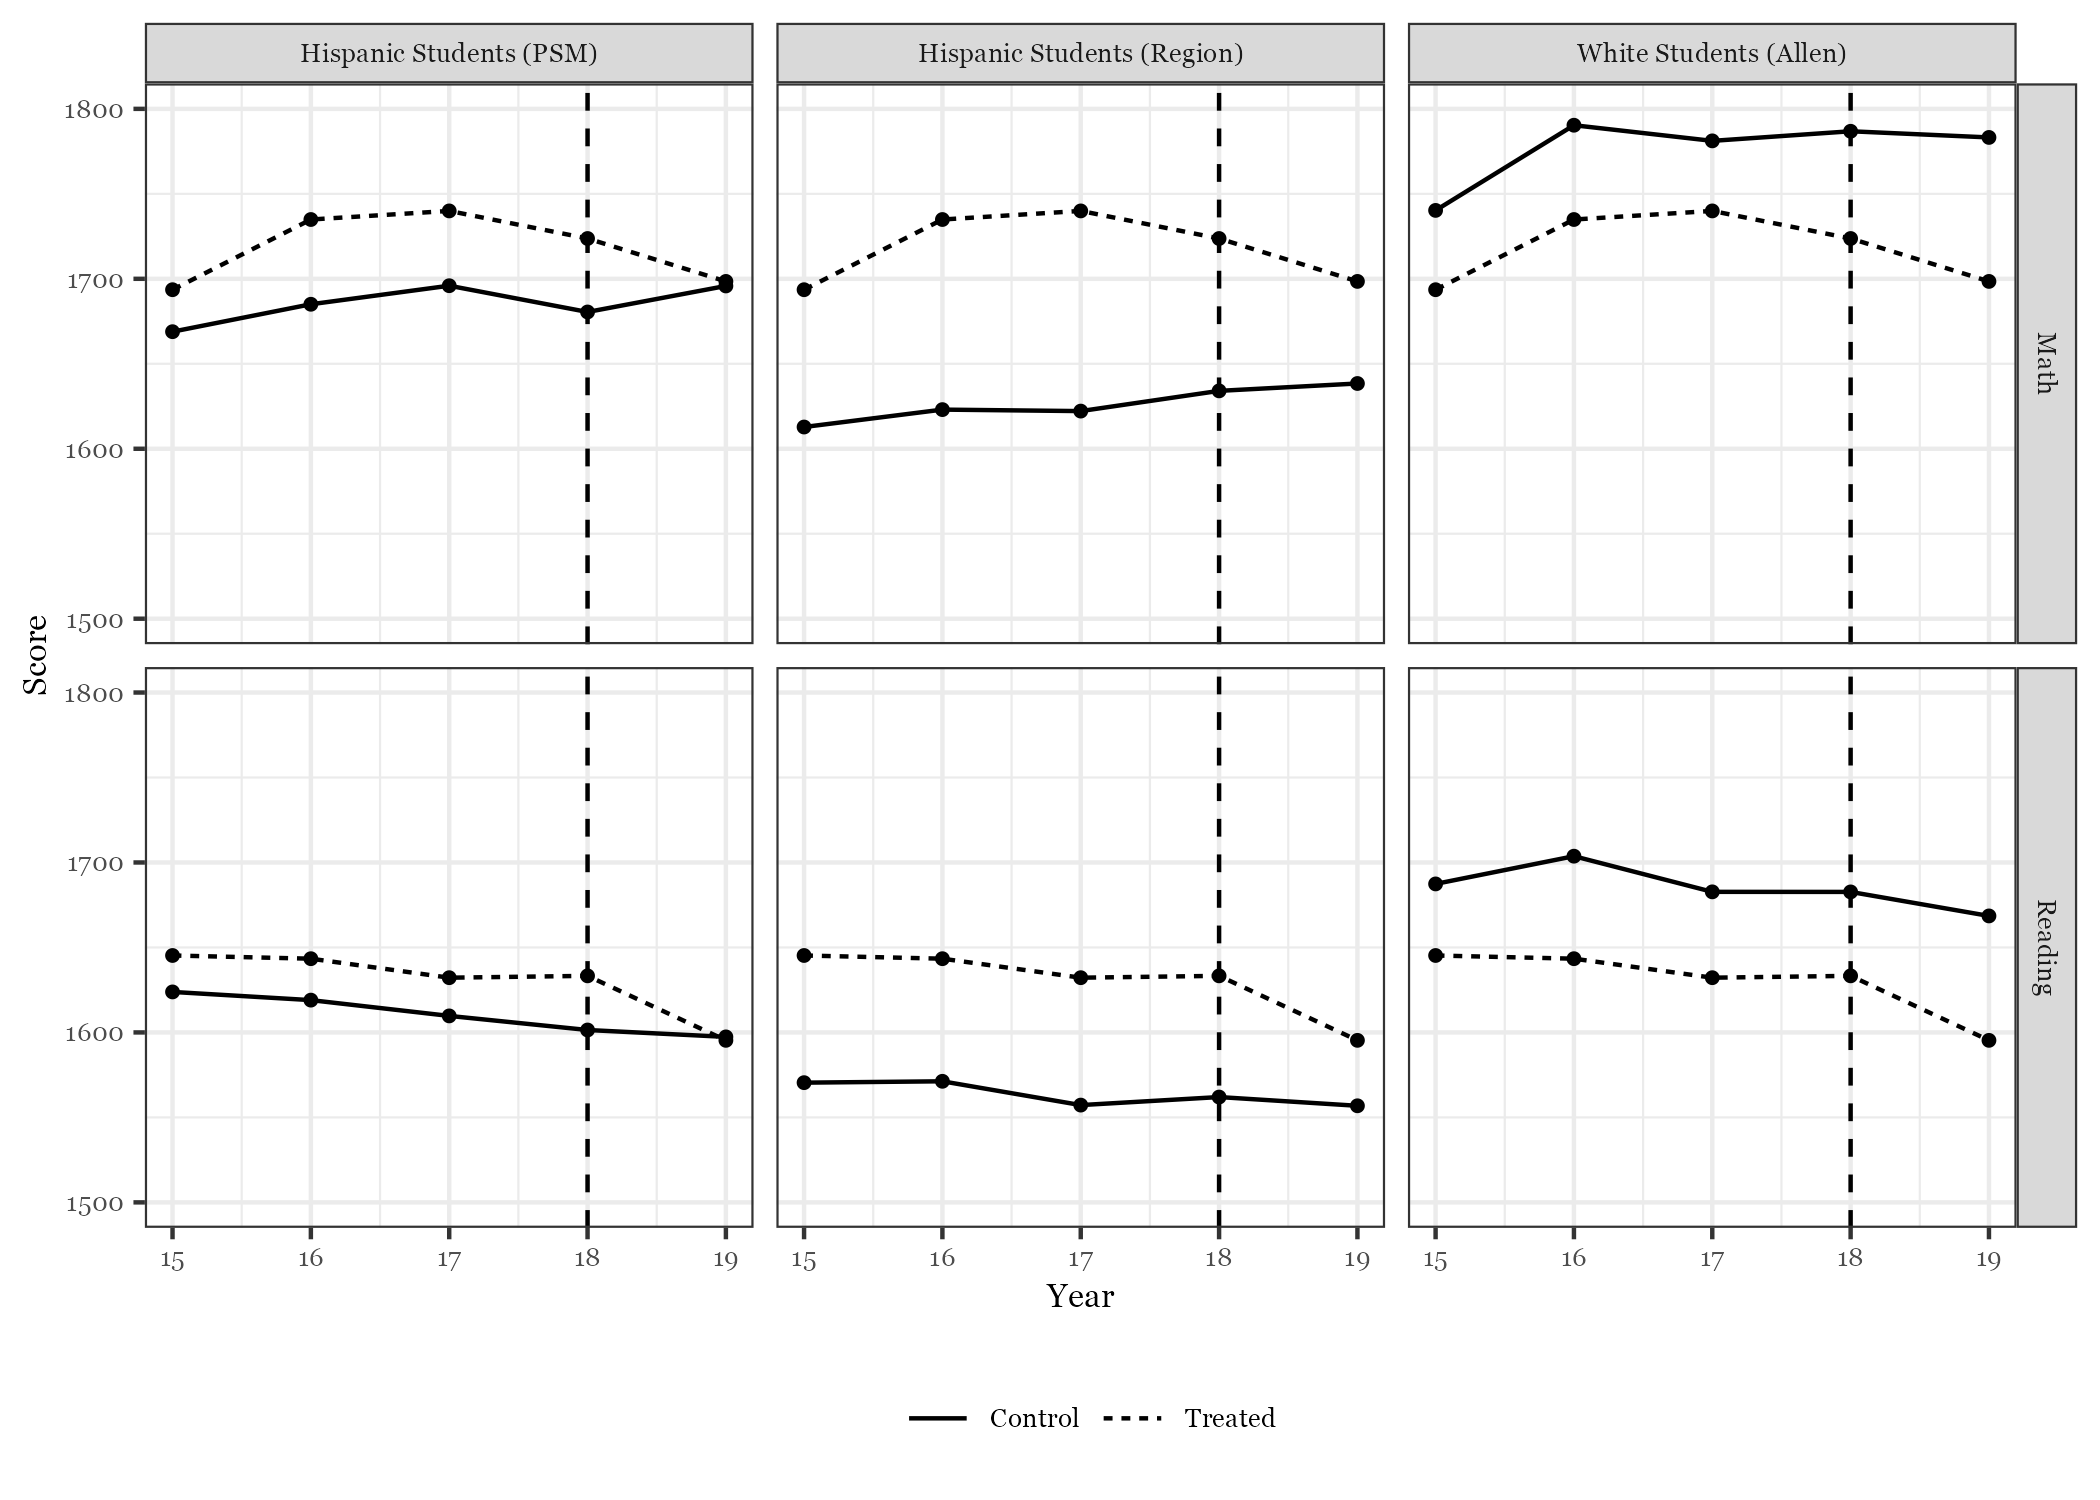
\includegraphics[scale=0.8]{did_trends_Score_math_reading.png}}
\end{figure}

\vspace{1ex}
\begin{figure}[H]
\caption{{Trends in math and reading passing rates across Hispanic students in Allen ISD and control groups}}
\centerline{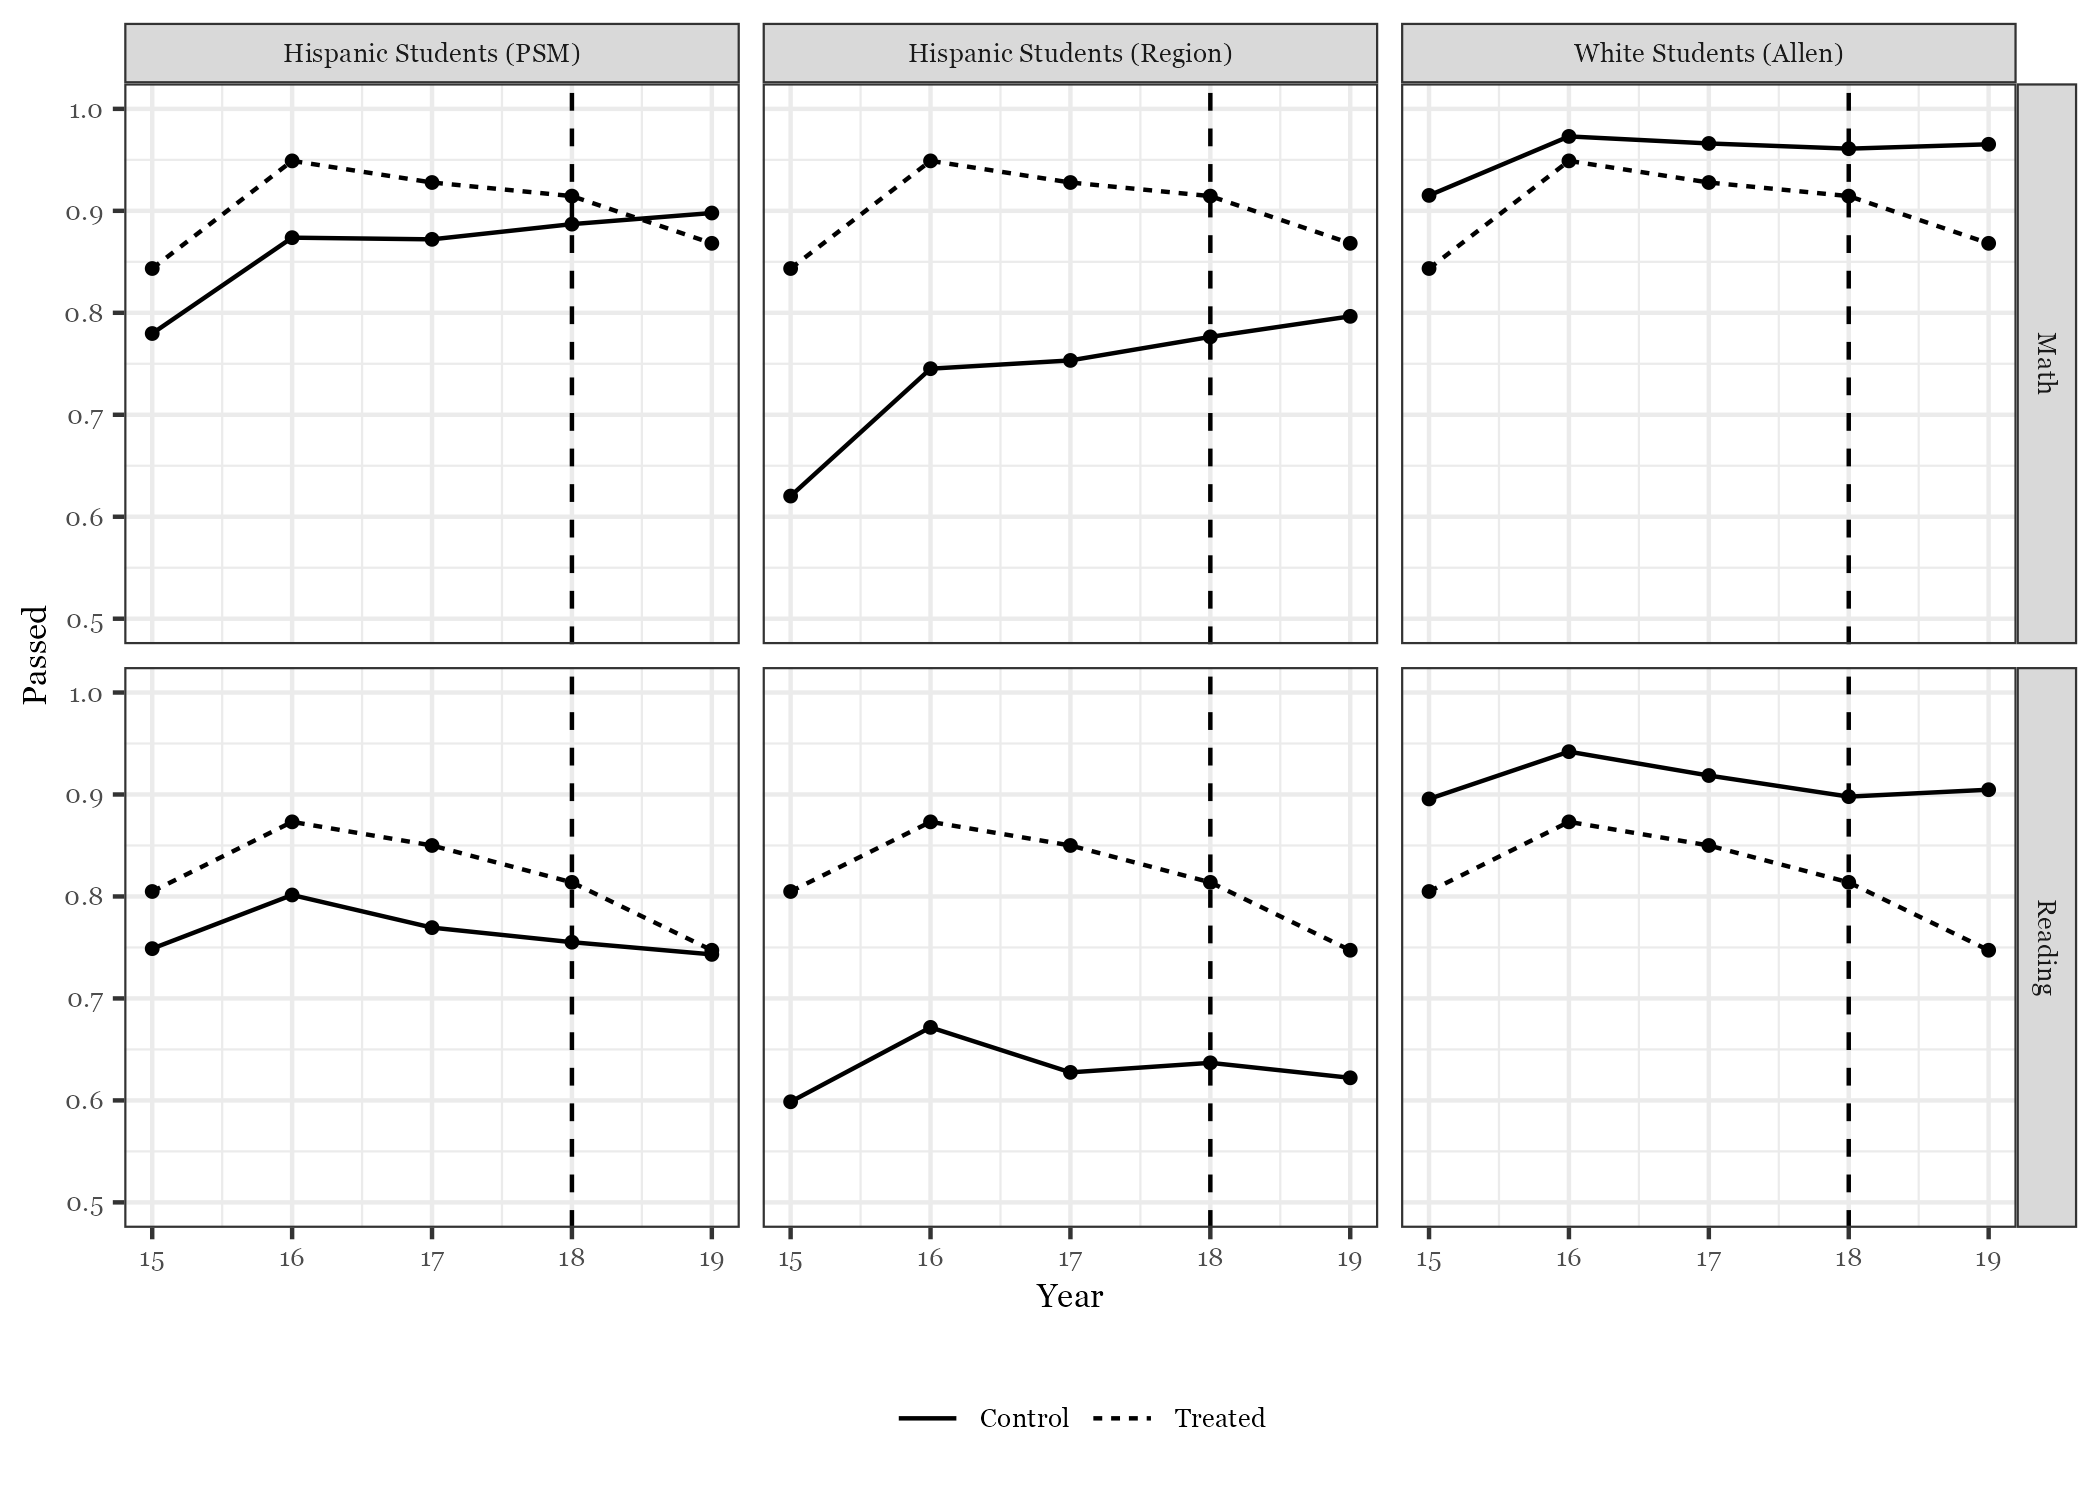
\includegraphics[scale=0.8]{did_trends_Passed_math_reading.png}}
\end{figure}

\vspace{1ex}
\begin{figure}[H]
\caption{{Estimates for the effect of workplace raids on academic performance using an event study specification}}
\centerline{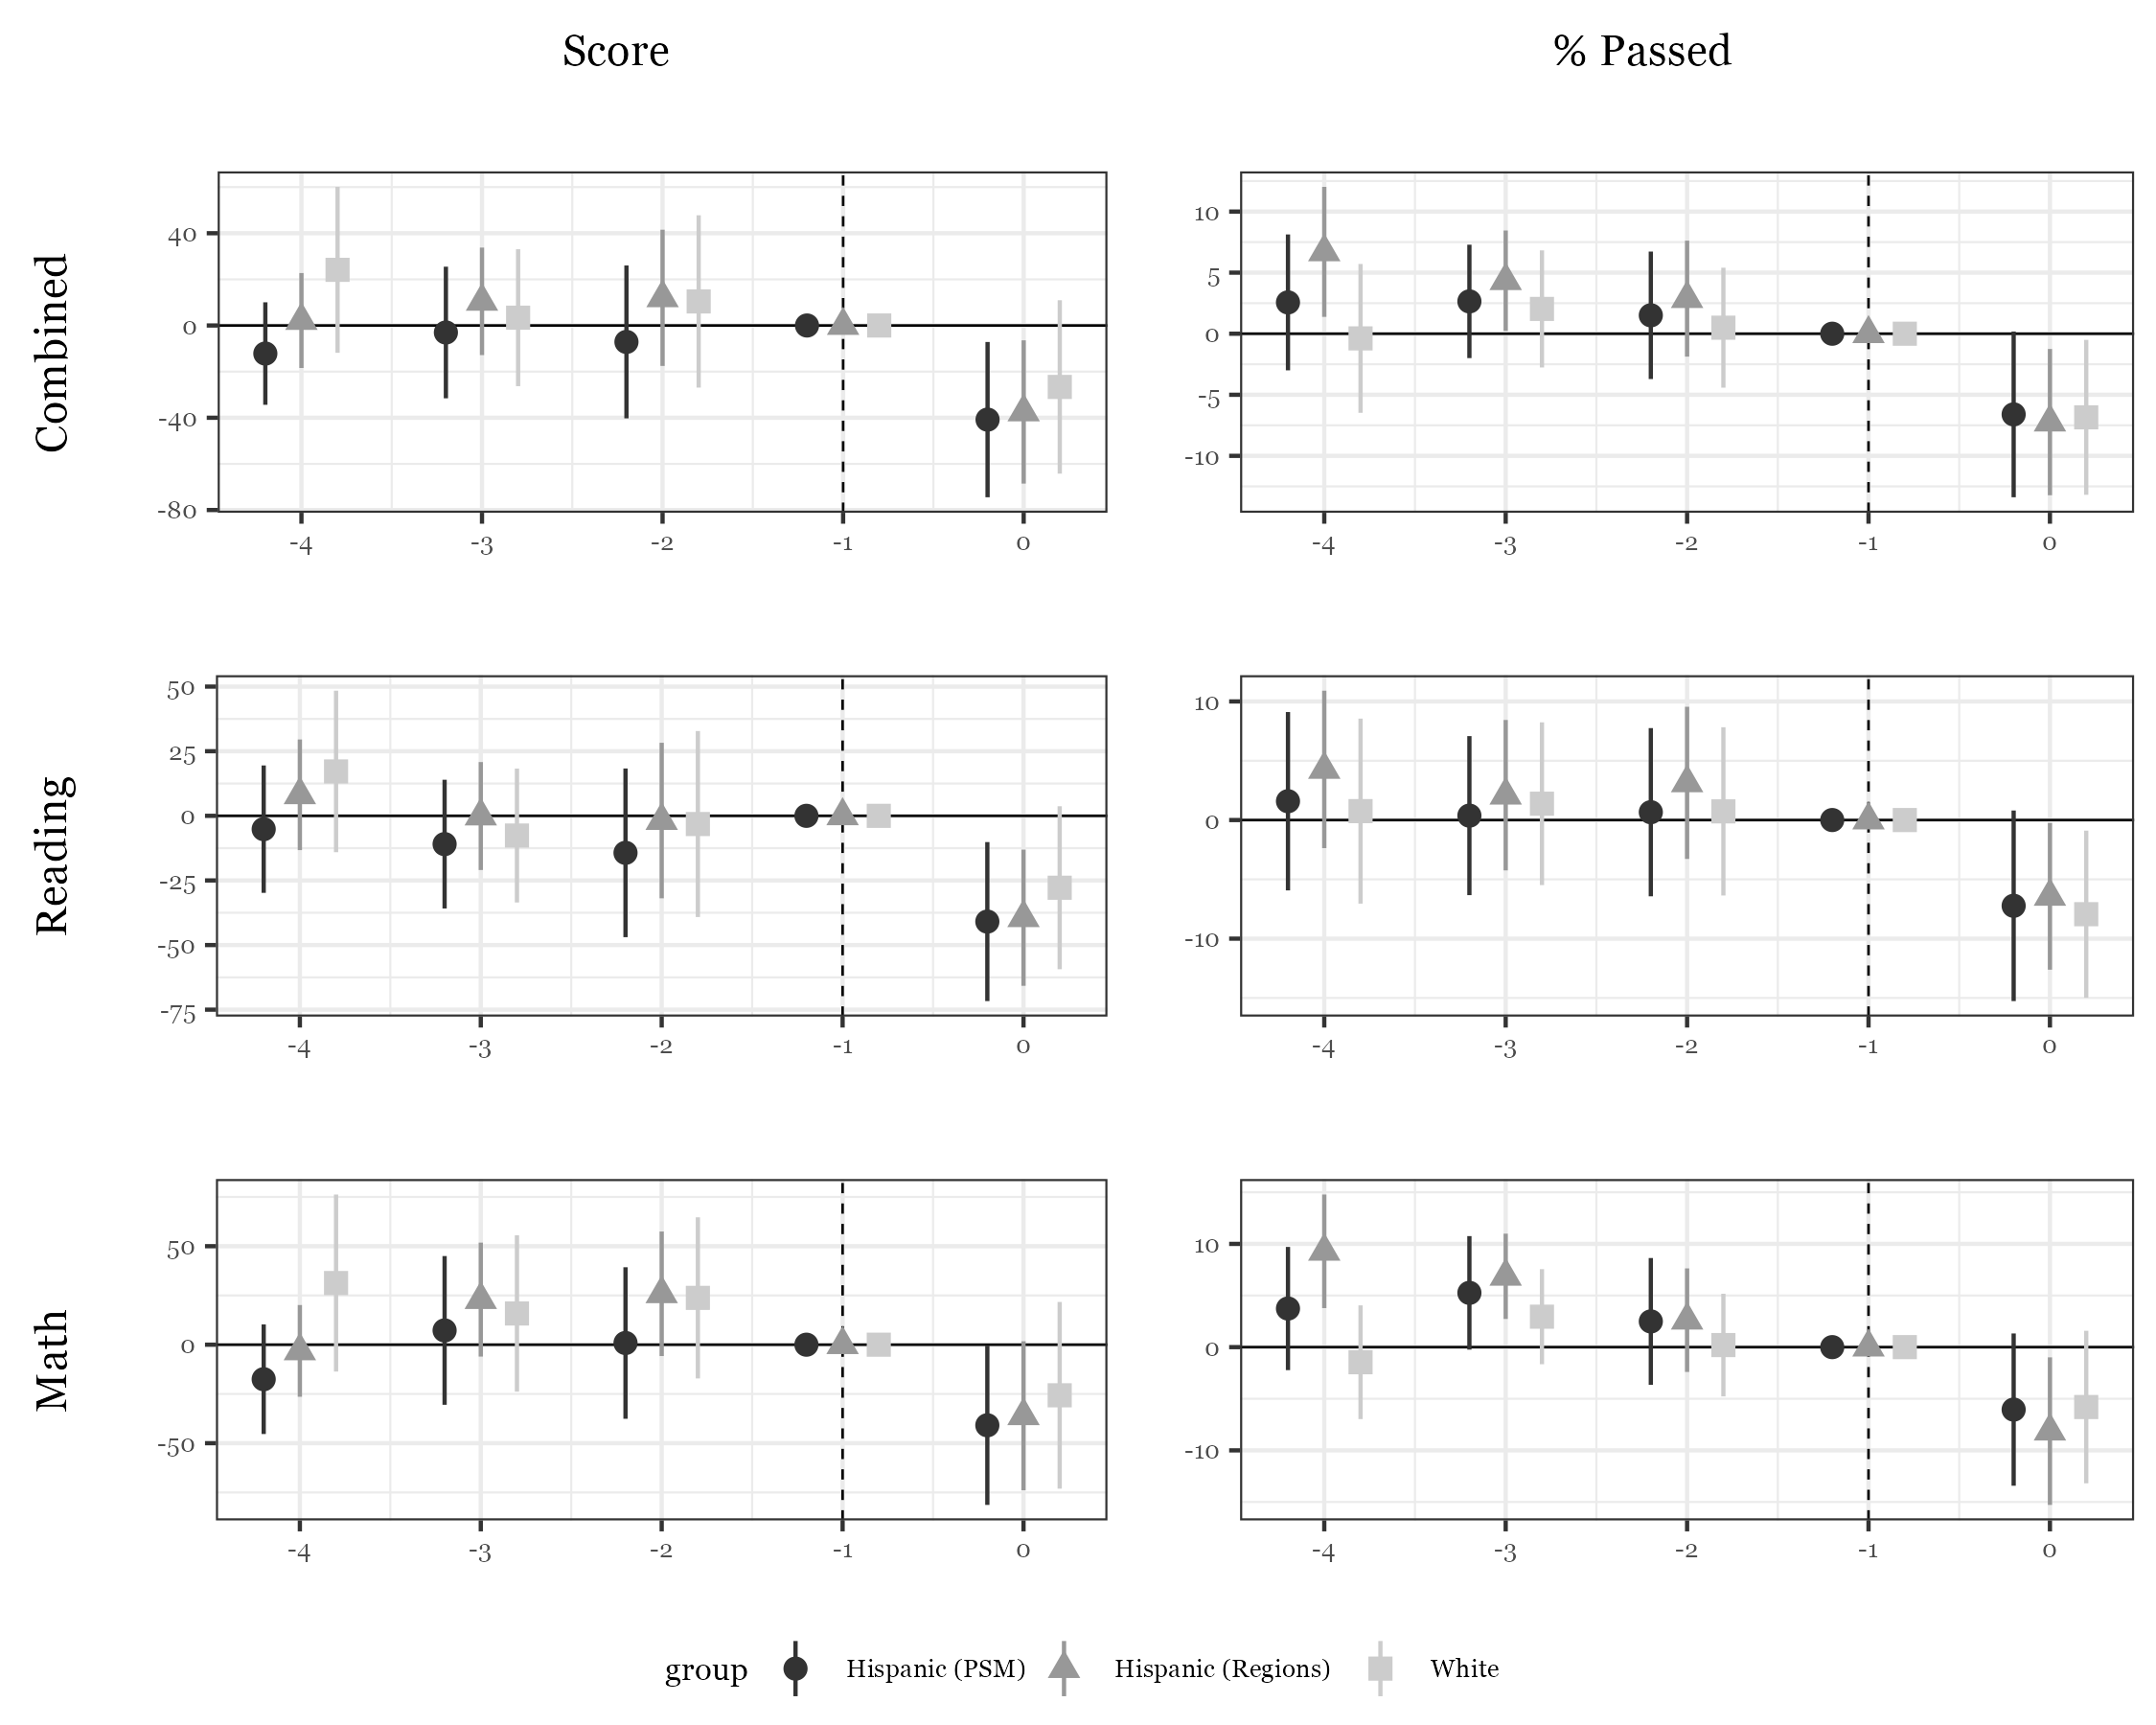
\includegraphics[scale=0.8]{event_study.png}}
\label{fig:performanceeventstudy}
\end{figure}


\vspace{1ex}
\begin{figure}[H]
\caption{{Estimated effect of workplace raid on math, reading, and combined test performance: alternative matching strategies}}
\centerline{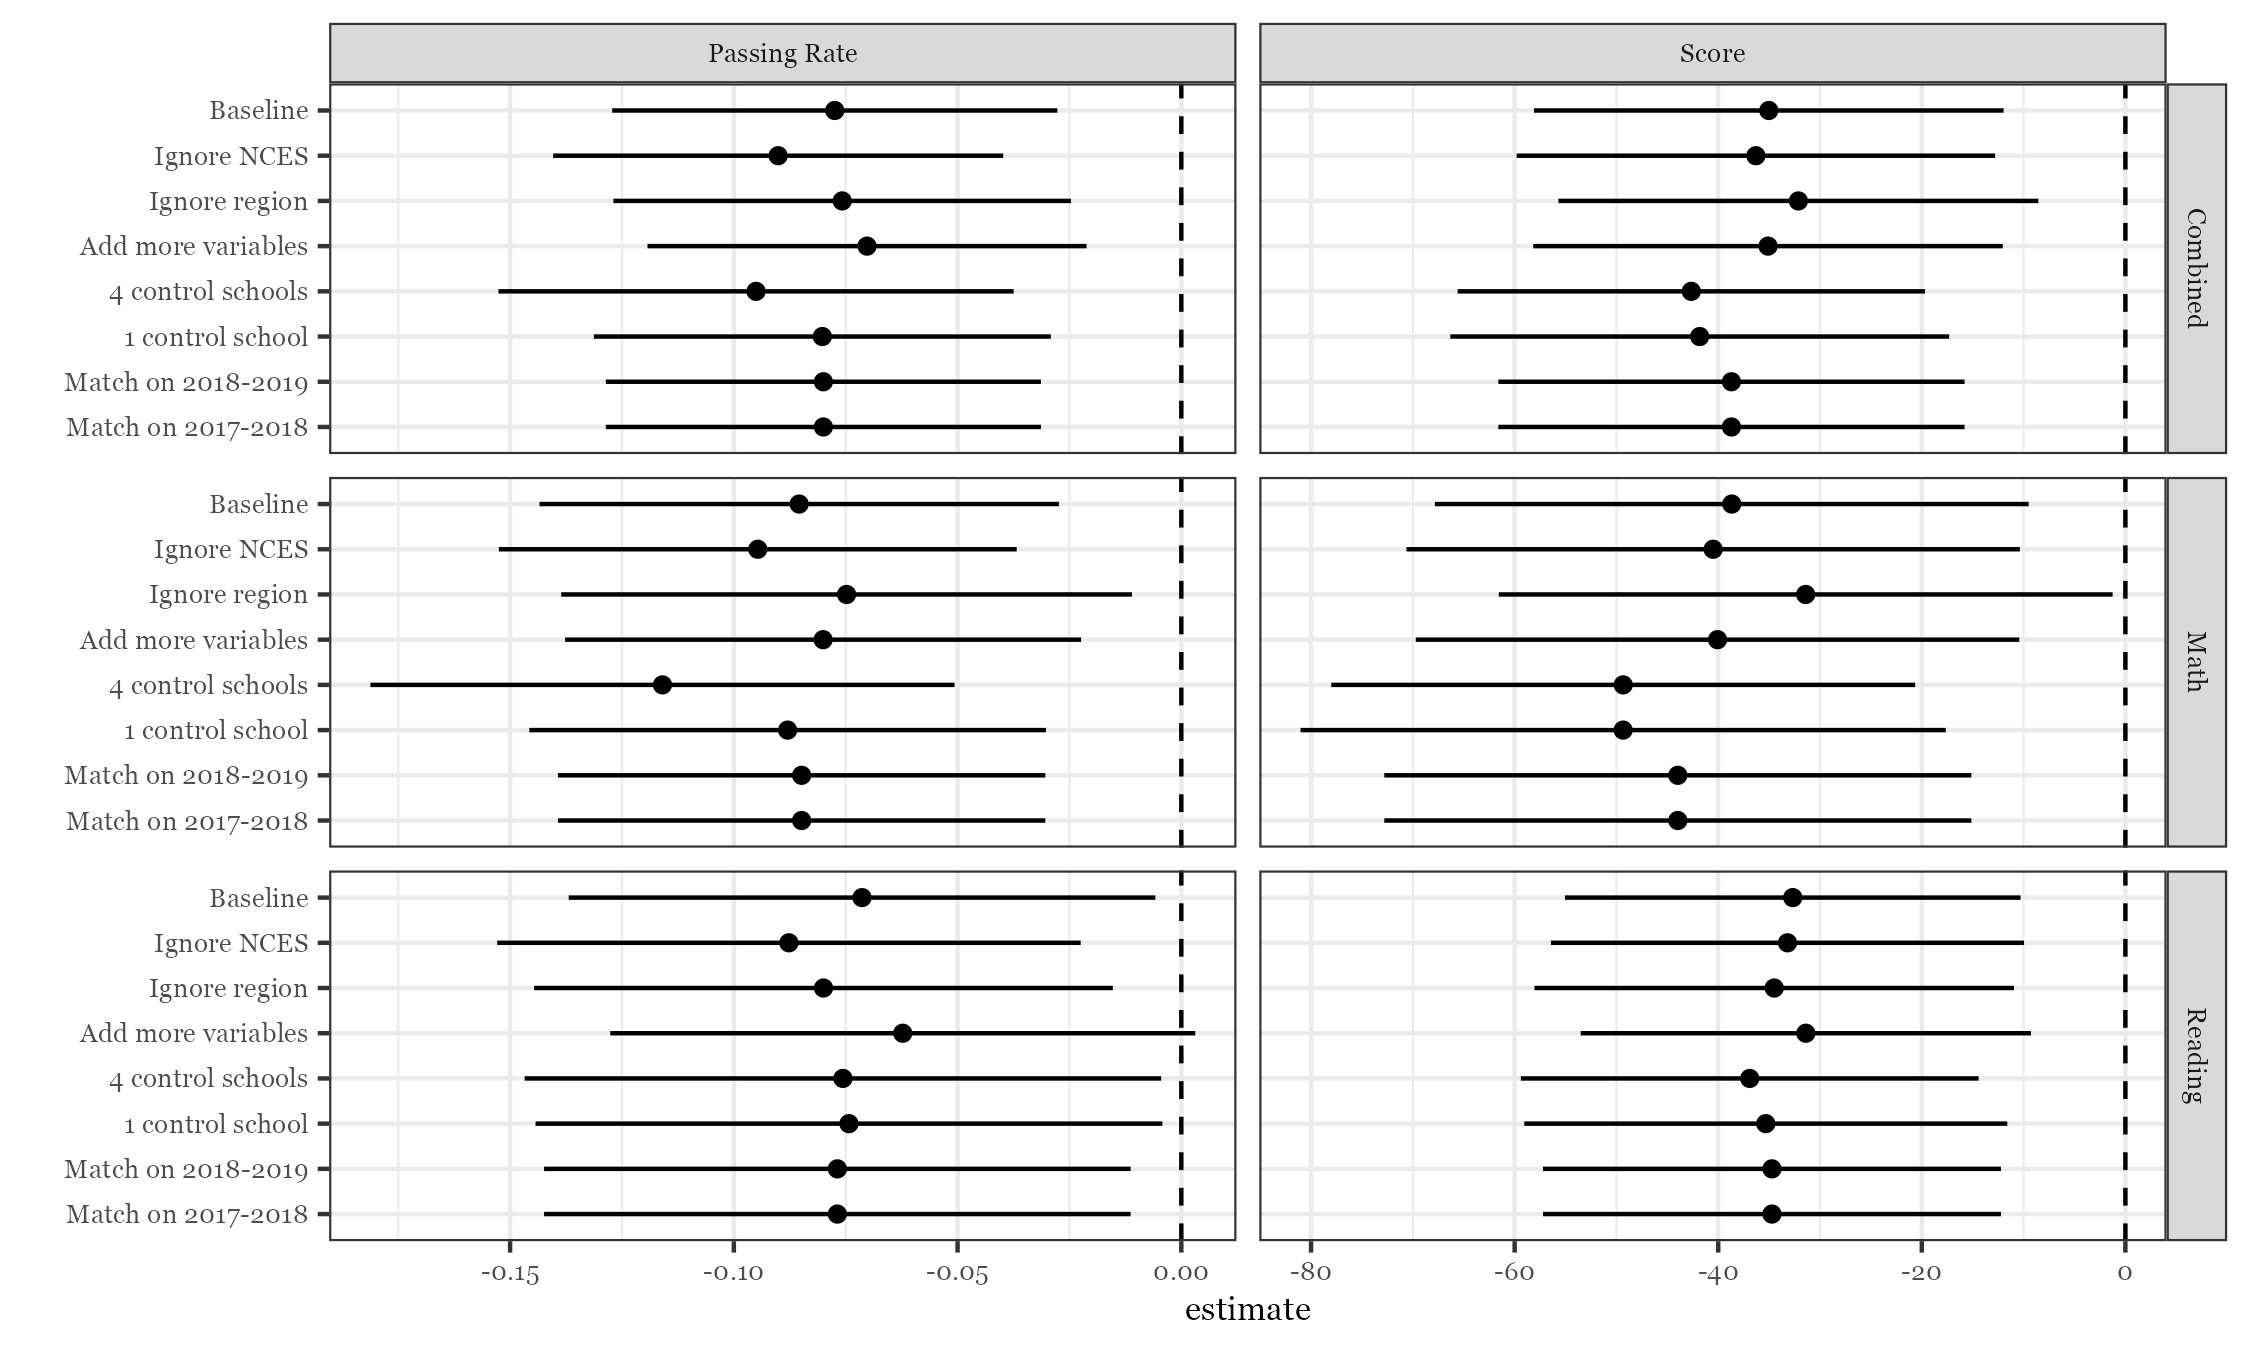
\includegraphics[scale=0.9]{psm_robustness.png}}
\label{fig:psmalt}
\end{figure}


\begin{figure}[H]
\caption{Change in academic performance 2018-2019 by distance between schools and site of workplace raid}
\centering
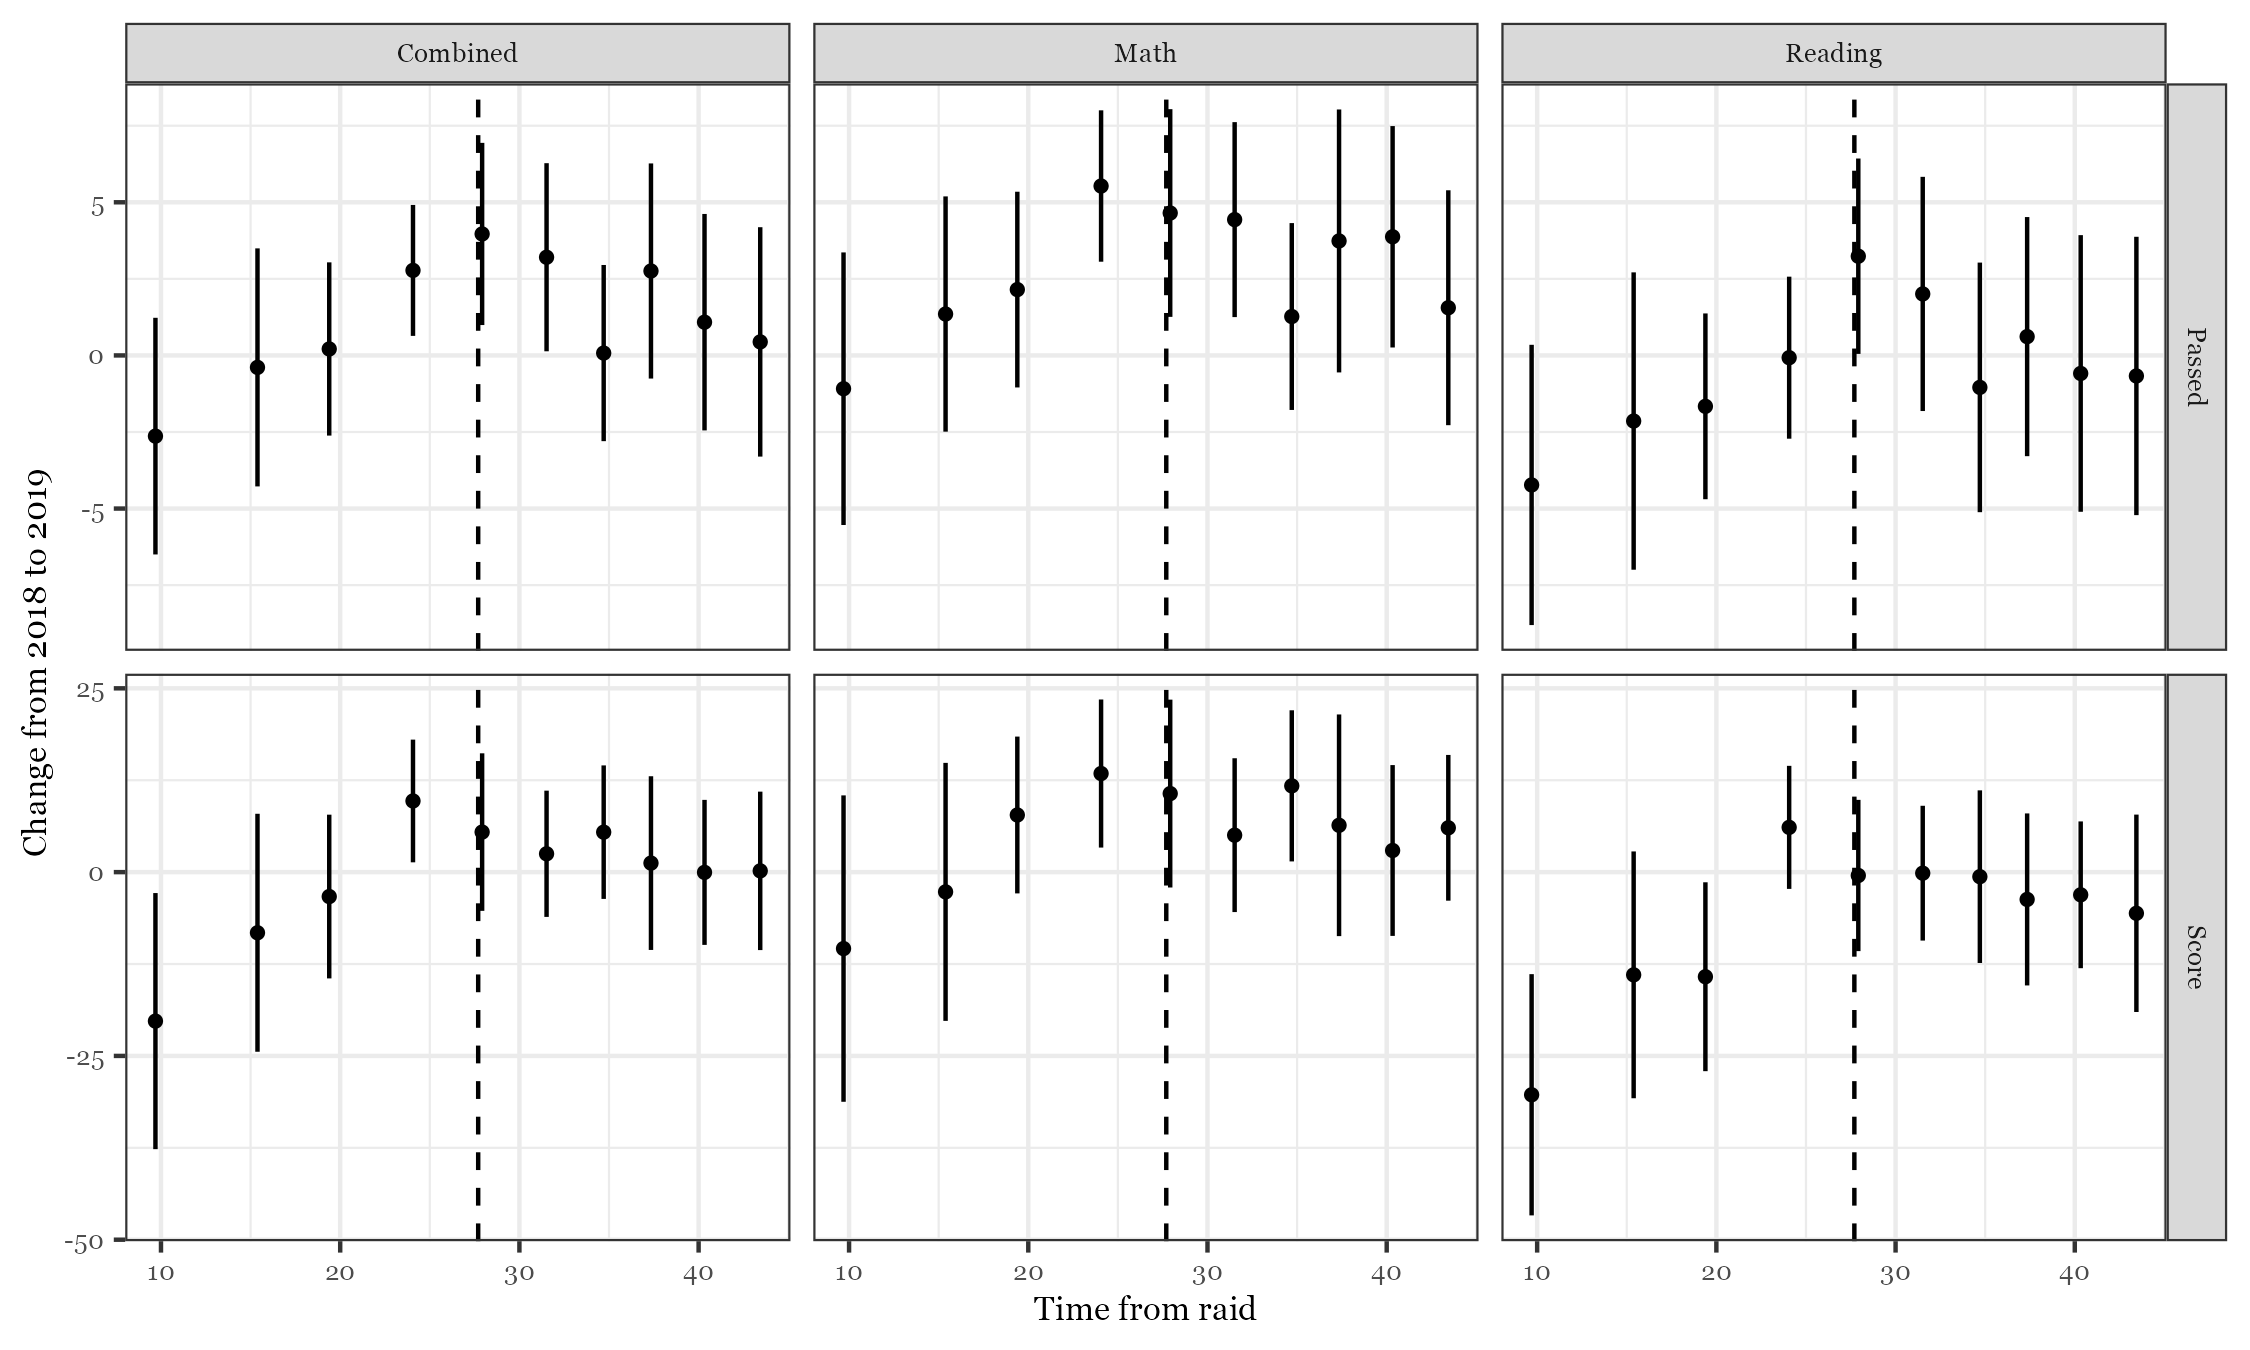
\includegraphics[scale=0.8]{distance_performance.png}
\caption*{\footnotesize \emph{Note:} This figure presents the change in score or passing rate for Hispanic students from 2018 to 2019 for each subject as well as for the combined test measure. The underlying data for the plot is at the school-level but I use a binscatter plot to make trends easier to visualize. For the binscatter, I divide the commuting time from the raid into 10 approximately equally sized bins and plot the conditional mean of the change in scores as well as the respective 95\% CI.} 
\label{fig:distanceperformance}
\end{figure}


\vspace{1ex}
\begin{figure}[H]
\caption{{Trends in year-over-year change in the number of visits recorded to schools in Allen ISD in the weeks before and after workplace raid}}
\centerline{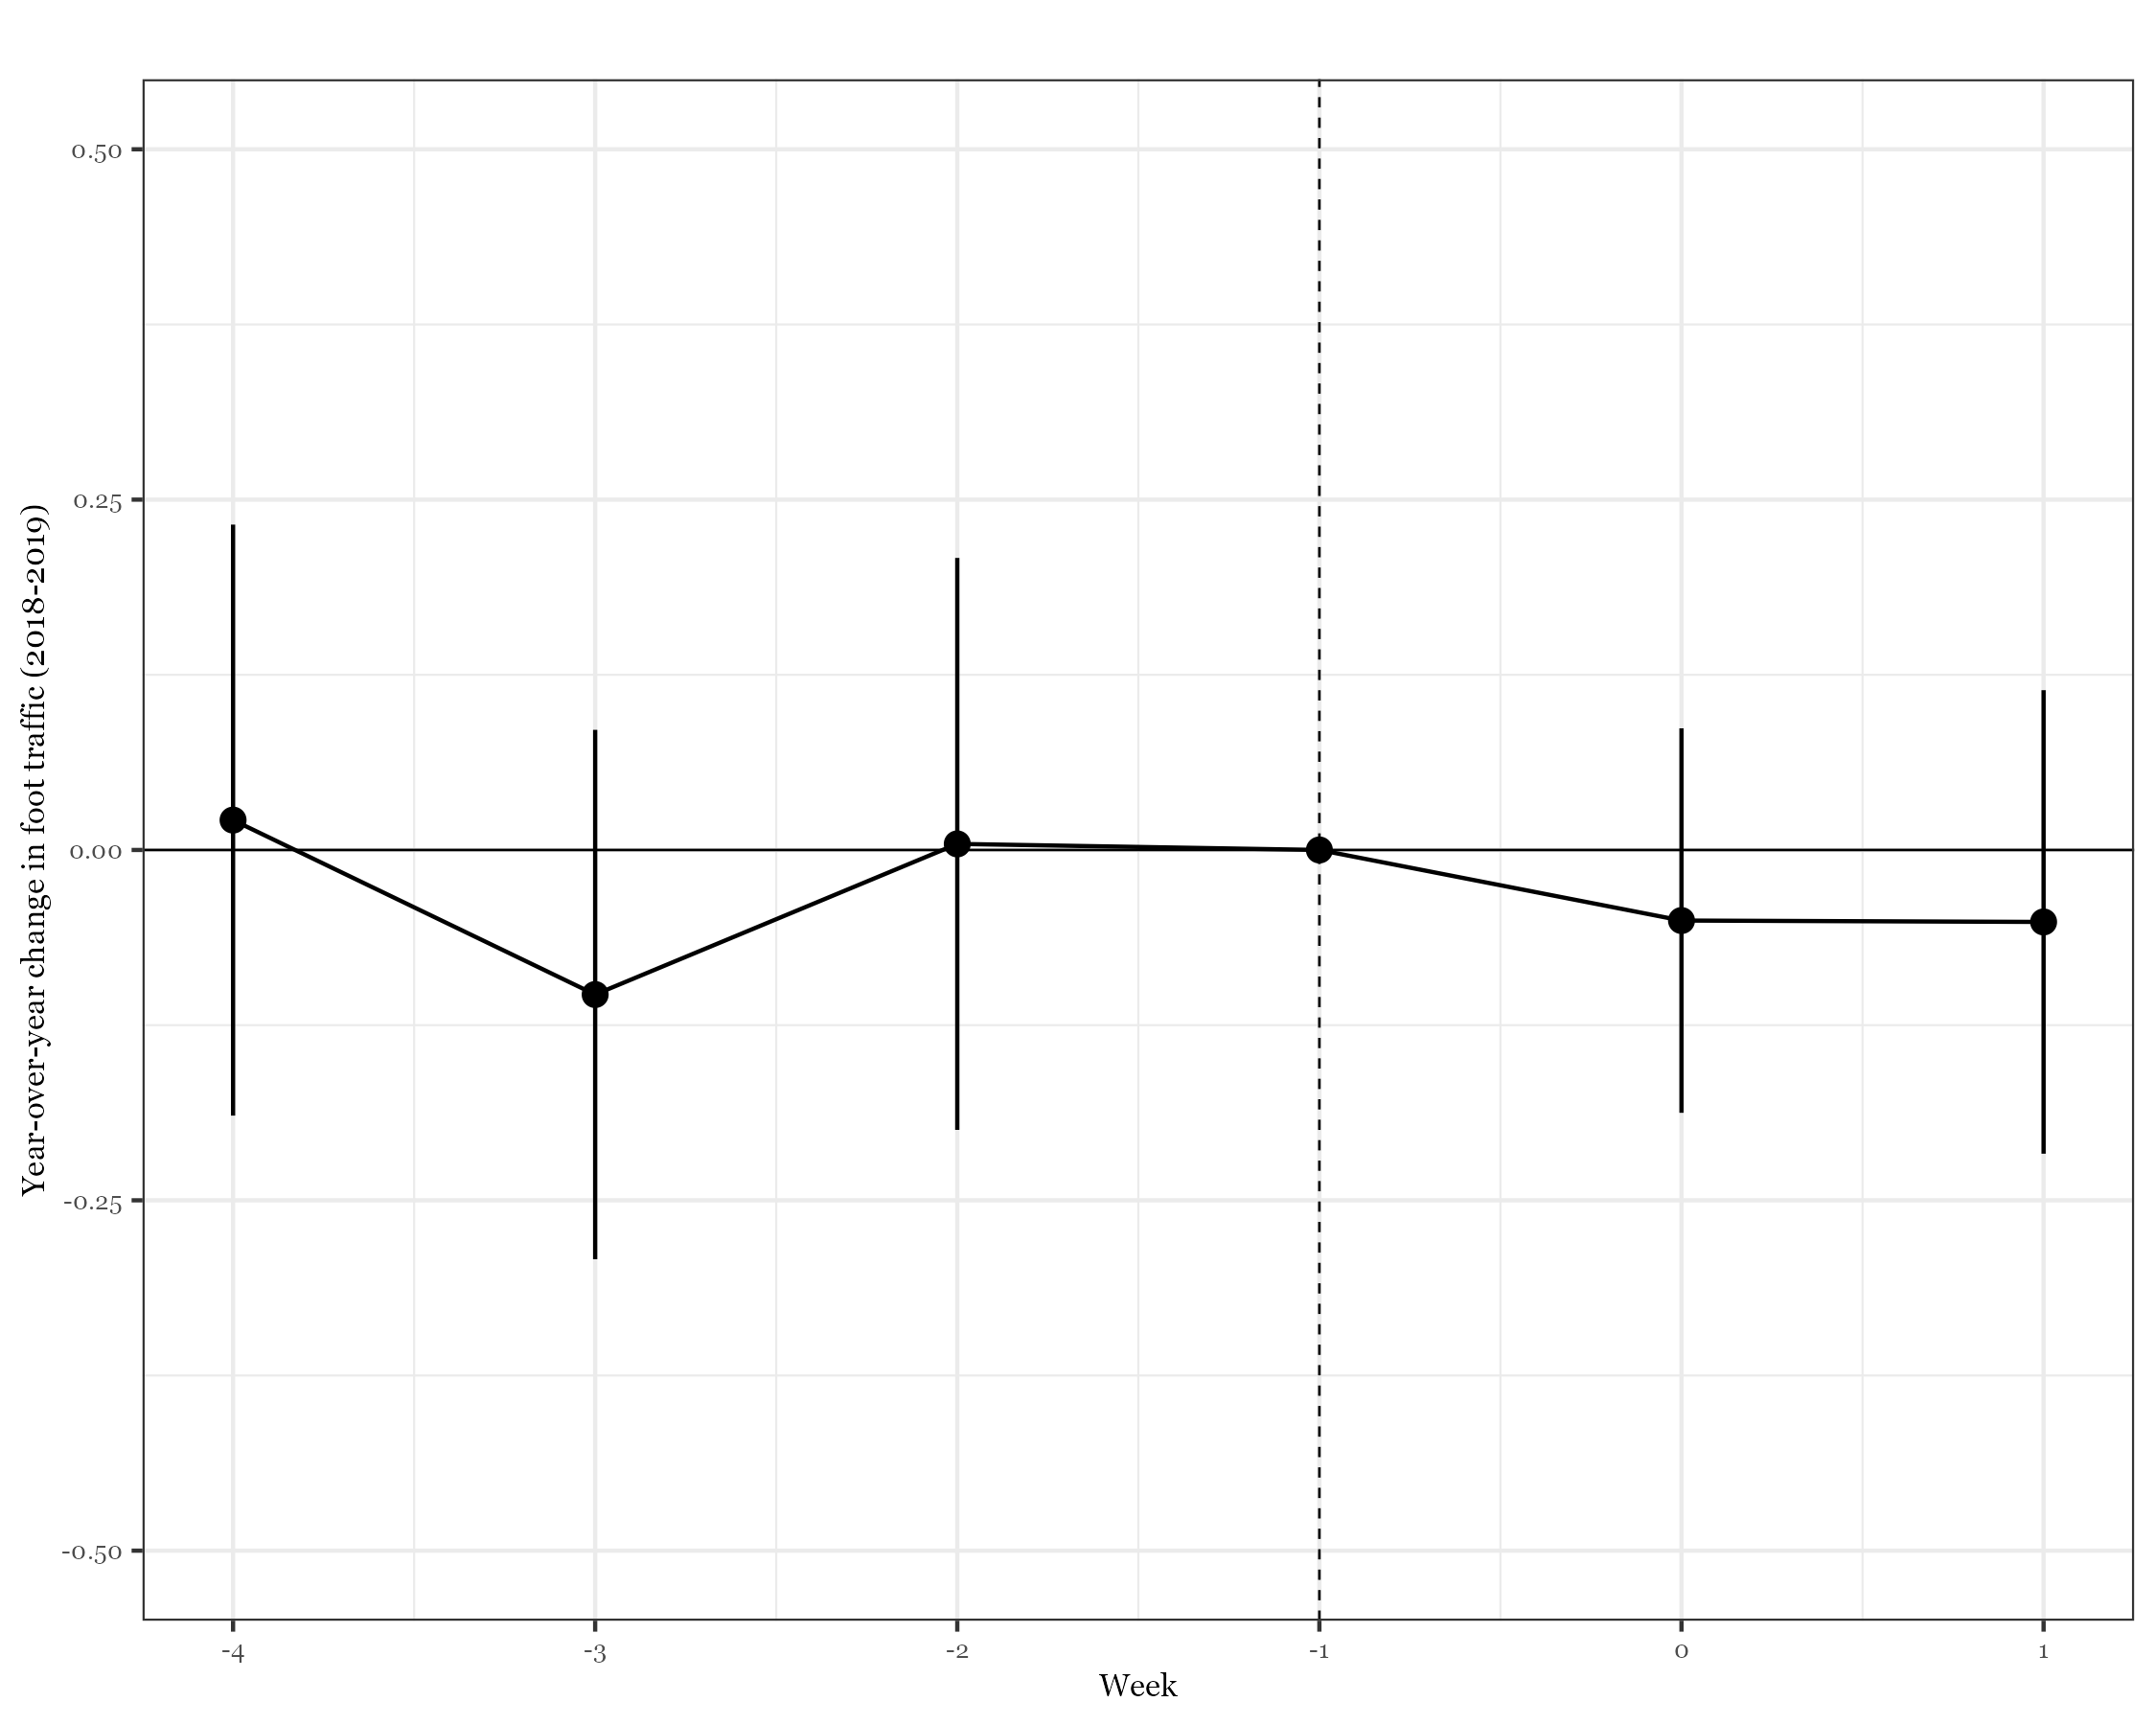
\includegraphics[scale=0.8]{safegraph_event_study.png}}
\end{figure}

\vspace{1ex}
\begin{figure}[H]
\caption{{Academic calendars Allen ISD 2017-2018 and 2018-2019}}
\centerline{\includegraphics[scale=0.05]{allen_academic_calendars.jpeg}}
\label{fig:allencal}
\end{figure}


\clearpage



\end{document}
